% This template is borrowed from the Reed College LaTeX thesis template. Most of the work
% for the document class was done by Sam Noble (SN), as well as this
% template. Later comments etc. by Ben Salzberg (BTS). Additional
% restructuring and APA support by Jess Youngberg (JY).
% Your comments and suggestions are more than welcome; please email
% them to cus@reed.edu
%
% See http://web.reed.edu/cis/help/latex.html for help. There are a
% great bunch of help pages there, with notes on
% getting started, bibtex, etc. Go there and read it if you're not
% already familiar with LaTeX.
%
% Any line that starts with a percent symbol is a comment.
% They won't show up in the document, and are useful for notes
% to yourself and explaining commands.
% Commenting also removes a line from the document;
% very handy for troubleshooting problems. -BTS

% As far as I know, this follows the requirements laid out in
% the 2002-2003 Senior Handbook. Ask a librarian to check the
% document before binding. -SN

%%
%% Preamble
%%
% \documentclass{<something>} must begin each LaTeX document
\documentclass[12pt,twoside]{deuthesis}
% Packages are extensions to the basic LaTeX functions. Whatever you
% want to typeset, there is probably a package out there for it.
% Chemistry (chemtex), screenplays, you name it.
% Check out CTAN to see: http://www.ctan.org/
%%
\usepackage{graphicx,latexsym}
\usepackage{amsmath}
\usepackage{amssymb,amsthm}
\usepackage{longtable,booktabs,setspace}
\usepackage{chemarr} %% Useful for one reaction arrow, useless if you're not a chem major
\usepackage[hyphens]{url}
% Added by CII
\usepackage{hyperref}
\usepackage{lmodern}
\usepackage{float}
\floatplacement{figure}{H}
% End of CII addition
\usepackage{rotating}

% Next line commented out by CII
%%% \usepackage{natbib}
% Comment out the natbib line above and uncomment the following two lines to use the new
% biblatex-chicago style, for Chicago A. Also make some changes at the end where the
% bibliography is included.
%\usepackage{biblatex-chicago}
%\bibliography{thesis}


% Added by CII (Thanks, Hadley!)
% Use ref for internal links
\renewcommand{\hyperref}[2][???]{\autoref{#1}}
\def\chapterautorefname{Chapter}
\def\sectionautorefname{Section}
\def\subsectionautorefname{Subsection}
% End of CII addition

% Added by CII
\usepackage{caption}
\captionsetup{width=5in}
% End of CII addition

% \usepackage{times} % other fonts are available like times, bookman, charter, palatino

% Syntax highlighting #22
  \usepackage{color}
  \usepackage{fancyvrb}
  \newcommand{\VerbBar}{|}
  \newcommand{\VERB}{\Verb[commandchars=\\\{\}]}
  \DefineVerbatimEnvironment{Highlighting}{Verbatim}{commandchars=\\\{\}}
  % Add ',fontsize=\small' for more characters per line
  \usepackage{framed}
  \definecolor{shadecolor}{RGB}{248,248,248}
  \newenvironment{Shaded}{\begin{snugshade}}{\end{snugshade}}
  \newcommand{\AlertTok}[1]{\textcolor[rgb]{0.94,0.16,0.16}{#1}}
  \newcommand{\AnnotationTok}[1]{\textcolor[rgb]{0.56,0.35,0.01}{\textbf{\textit{#1}}}}
  \newcommand{\AttributeTok}[1]{\textcolor[rgb]{0.13,0.29,0.53}{#1}}
  \newcommand{\BaseNTok}[1]{\textcolor[rgb]{0.00,0.00,0.81}{#1}}
  \newcommand{\BuiltInTok}[1]{#1}
  \newcommand{\CharTok}[1]{\textcolor[rgb]{0.31,0.60,0.02}{#1}}
  \newcommand{\CommentTok}[1]{\textcolor[rgb]{0.56,0.35,0.01}{\textit{#1}}}
  \newcommand{\CommentVarTok}[1]{\textcolor[rgb]{0.56,0.35,0.01}{\textbf{\textit{#1}}}}
  \newcommand{\ConstantTok}[1]{\textcolor[rgb]{0.56,0.35,0.01}{#1}}
  \newcommand{\ControlFlowTok}[1]{\textcolor[rgb]{0.13,0.29,0.53}{\textbf{#1}}}
  \newcommand{\DataTypeTok}[1]{\textcolor[rgb]{0.13,0.29,0.53}{#1}}
  \newcommand{\DecValTok}[1]{\textcolor[rgb]{0.00,0.00,0.81}{#1}}
  \newcommand{\DocumentationTok}[1]{\textcolor[rgb]{0.56,0.35,0.01}{\textbf{\textit{#1}}}}
  \newcommand{\ErrorTok}[1]{\textcolor[rgb]{0.64,0.00,0.00}{\textbf{#1}}}
  \newcommand{\ExtensionTok}[1]{#1}
  \newcommand{\FloatTok}[1]{\textcolor[rgb]{0.00,0.00,0.81}{#1}}
  \newcommand{\FunctionTok}[1]{\textcolor[rgb]{0.13,0.29,0.53}{\textbf{#1}}}
  \newcommand{\ImportTok}[1]{#1}
  \newcommand{\InformationTok}[1]{\textcolor[rgb]{0.56,0.35,0.01}{\textbf{\textit{#1}}}}
  \newcommand{\KeywordTok}[1]{\textcolor[rgb]{0.13,0.29,0.53}{\textbf{#1}}}
  \newcommand{\NormalTok}[1]{#1}
  \newcommand{\OperatorTok}[1]{\textcolor[rgb]{0.81,0.36,0.00}{\textbf{#1}}}
  \newcommand{\OtherTok}[1]{\textcolor[rgb]{0.56,0.35,0.01}{#1}}
  \newcommand{\PreprocessorTok}[1]{\textcolor[rgb]{0.56,0.35,0.01}{\textit{#1}}}
  \newcommand{\RegionMarkerTok}[1]{#1}
  \newcommand{\SpecialCharTok}[1]{\textcolor[rgb]{0.81,0.36,0.00}{\textbf{#1}}}
  \newcommand{\SpecialStringTok}[1]{\textcolor[rgb]{0.31,0.60,0.02}{#1}}
  \newcommand{\StringTok}[1]{\textcolor[rgb]{0.31,0.60,0.02}{#1}}
  \newcommand{\VariableTok}[1]{\textcolor[rgb]{0.00,0.00,0.00}{#1}}
  \newcommand{\VerbatimStringTok}[1]{\textcolor[rgb]{0.31,0.60,0.02}{#1}}
  \newcommand{\WarningTok}[1]{\textcolor[rgb]{0.56,0.35,0.01}{\textbf{\textit{#1}}}}

% To pass between YAML and LaTeX the dollar signs are added by CII
\title{Değişim Noktası Belirleme Yöntemleri ve Uygulamaları}
%\author{Pelin PEKERMerve AKEdanur Binnaz DURSUNAhmet ÇALI} %Tek yazar için
\author{Pelin PEKER \\ Merve AK \\ Edanur Binnaz DURSUN \\ Ahmet ÇALI} %Çok yazar için
% The month and year that you submit your FINAL draft TO THE LIBRARY (May or December)
\date{May 2024}
\division{İSTATİSTİK BÖLÜMÜ}
\advisor{Dr.~Engin YILDIZTEPE}
\institution{FEN FAKÜLTESİ}
\degree{Bitirme Projesi Raporu}
%If you have two advisors for some reason, you can use the following
% Uncommented out by CII
% End of CII addition

%%% Remember to use the correct department!
\department{İstatistik Bölümü}
% if you're writing a thesis in an interdisciplinary major,
% uncomment the line below and change the text as appropriate.
% check the Senior Handbook if unsure.
%\thedivisionof{The Established Interdisciplinary Committee for}
% if you want the approval page to say "Approved for the Committee",
% uncomment the next line
%\approvedforthe{Committee}

% Added by CII
%%% Copied from knitr
%% maxwidth is the original width if it's less than linewidth
%% otherwise use linewidth (to make sure the graphics do not exceed the margin)
\makeatletter
\def\maxwidth{ %
  \ifdim\Gin@nat@width>\linewidth
    \linewidth
  \else
    \Gin@nat@width
  \fi
}
\makeatother

\renewcommand{\contentsname}{Table of Contents}
% End of CII addition

\setlength{\parskip}{0pt}

% Added by CII

\providecommand{\tightlist}{%
  \setlength{\itemsep}{0pt}\setlength{\parskip}{0pt}}

\Acknowledgements{
Tüm çalışma süresince yönlendiriciliği, katkıları ve yardımları ile yanımızda olan danışmanımız Dr.~Engin YILDIZTEPE 'ye ve böyle bir çalışmayı yapmamız için bize fırsat tanıyan Dokuz Eylül Üniversitesi Fen Fakültesi İstatistik Bölümüne teşekkür ederiz.\\
\strut \\
\strut \\
Pelin PEKER\\
Merve AK\\
Edanur Binnaz DURSUN\\
Ahmet ÇALI\\
}

\Dedication{

}

\Preface{
``Değişim Noktası Belirleme Yöntemleri ve Uygulamaları'' başlıklı bitirme projesi raporu tarafıgitmdan okunmuş, kapsamı ve niteliği açısından bir Bitirme Projesi raporu olarak kabul edilmiştir.\\
\strut \\
\strut \\
Dr.~Engin YILDIZTEPE
}

\AbstractTR{
Değişim noktası verilerde meydana gelen beklenmedik anlamlı değişiklikler olarak tanımlanabilir. Değişim noktası tespit yöntemleri bu noktaları istatistiksel tekniklerle bulmayı amaçlar. Değişim noktası analizi finans, kalite kontrol, ağ analizi gibi çok farklı alanlarda kullanılmaktadır. Bu çalışmada değişim noktası tespit yöntemleri incelenmiştir. Çalışma kapsamında AMOC, BinSeg, parçalı regresyon, PELT ve Prophet algoritmaları kullanılmıştır. Algoritmaların uygulamadaki performanslarını belirlemek amacıyla yirmi yapay ve on bir gerçek veri kullanılmıştır. Performanslar F1 puanı ve kapsama ölçütü kullanılarak değerlendirilmiştir. F1 puanına göre en başarılı sonuçlar yapay verilerde BinSeg ile, gerçek verilerde parçalı regresyon ile alınmıştır. Kapsama ölçütüne göre ise yapay verilerde BinSeg ve parçalı regresyon, gerçek verilerde parçalı regresyon ile en iyi sonuçlar elde edilmiştir. Değişim noktası içeren yapay veri üretmek ve bahsedilen algoritmaları uygulayabilmek amacıyla bir RShiny web uygulaması geliştirilmiştir. Çalışmada R ve Python programlama dilleri kullanılmıştır.\\
\strut \\

\textbf{Anahtar Kelimeler:} Değişim noktası, AMOC, BinSeg, PELT, Prophet, Parçalı Regresyon, R shiny
}

\Abstract{
Change points can be defined as unexpected significant changes occurring in data. Change point detection methods aim to identify these points using statistical techniques. Change point analysis is utilized in various fields such as finance, quality control, and network analysis. In this study, change point detection methods were examined. AMOC, BinSeg, Segmented Regression, PELT, and Prophet algorithms were used within the scope of the study. To determine the performance of the algorithms in application, twenty artificial and eleven real datasets were employed. Performance was evaluated using the F1 score and cover metric. According to the F1 score, the most successful results were obtained with BinSeg on artificial data and with Segmented Regression on real data. Regarding the cover metric, BinSeg and Segmented Regression yielded the best results on artificial data, while Segmented Regression performed the best on real data. To generate artificial data containing change points and apply the mentioned algorithms, an R Shiny web application was developed. Both R and Python programming languages were used in the study.\\
\strut \\

\textbf{Keywords:} Changepoint, AMOC, BinSeg, Pelt, Prophet, Segmented Regression, R Shiny
}


% End of CII addition
%%
%% End Preamble
%%
%

\begin{document}

% Everything below added by CII
  \maketitle

\frontmatter % this stuff will be roman-numbered
\pagestyle{empty} % this removes page numbers from the frontmatter

\begin{preface}
	``Değişim Noktası Belirleme Yöntemleri ve Uygulamaları'' başlıklı bitirme projesi raporu tarafıgitmdan okunmuş, kapsamı ve niteliği açısından bir Bitirme Projesi raporu olarak kabul edilmiştir.\\
\strut \\
\strut \\
Dr.~Engin YILDIZTEPE
\end{preface}

  \begin{acknowledgements}
    Tüm çalışma süresince yönlendiriciliği, katkıları ve yardımları ile yanımızda olan danışmanımız Dr.~Engin YILDIZTEPE 'ye ve böyle bir çalışmayı yapmamız için bize fırsat tanıyan Dokuz Eylül Üniversitesi Fen Fakültesi İstatistik Bölümüne teşekkür ederiz.\\
    \strut \\
    \strut \\
    Pelin PEKER\\
    Merve AK\\
    Edanur Binnaz DURSUN\\
    Ahmet ÇALI\\
  \end{acknowledgements}

\begin{abstractTR}
	Değişim noktası verilerde meydana gelen beklenmedik anlamlı değişiklikler olarak tanımlanabilir. Değişim noktası tespit yöntemleri bu noktaları istatistiksel tekniklerle bulmayı amaçlar. Değişim noktası analizi finans, kalite kontrol, ağ analizi gibi çok farklı alanlarda kullanılmaktadır. Bu çalışmada değişim noktası tespit yöntemleri incelenmiştir. Çalışma kapsamında AMOC, BinSeg, parçalı regresyon, PELT ve Prophet algoritmaları kullanılmıştır. Algoritmaların uygulamadaki performanslarını belirlemek amacıyla yirmi yapay ve on bir gerçek veri kullanılmıştır. Performanslar F1 puanı ve kapsama ölçütü kullanılarak değerlendirilmiştir. F1 puanına göre en başarılı sonuçlar yapay verilerde BinSeg ile, gerçek verilerde parçalı regresyon ile alınmıştır. Kapsama ölçütüne göre ise yapay verilerde BinSeg ve parçalı regresyon, gerçek verilerde parçalı regresyon ile en iyi sonuçlar elde edilmiştir. Değişim noktası içeren yapay veri üretmek ve bahsedilen algoritmaları uygulayabilmek amacıyla bir RShiny web uygulaması geliştirilmiştir. Çalışmada R ve Python programlama dilleri kullanılmıştır.\\
\strut \\

\textbf{Anahtar Kelimeler:} Değişim noktası, AMOC, BinSeg, PELT, Prophet, Parçalı Regresyon, R shiny
\end{abstractTR}

\begin{abstract}
	Change points can be defined as unexpected significant changes occurring in data. Change point detection methods aim to identify these points using statistical techniques. Change point analysis is utilized in various fields such as finance, quality control, and network analysis. In this study, change point detection methods were examined. AMOC, BinSeg, Segmented Regression, PELT, and Prophet algorithms were used within the scope of the study. To determine the performance of the algorithms in application, twenty artificial and eleven real datasets were employed. Performance was evaluated using the F1 score and cover metric. According to the F1 score, the most successful results were obtained with BinSeg on artificial data and with Segmented Regression on real data. Regarding the cover metric, BinSeg and Segmented Regression yielded the best results on artificial data, while Segmented Regression performed the best on real data. To generate artificial data containing change points and apply the mentioned algorithms, an R Shiny web application was developed. Both R and Python programming languages were used in the study.\\
\strut \\

\textbf{Keywords:} Changepoint, AMOC, BinSeg, Pelt, Prophet, Segmented Regression, R Shiny
\end{abstract}


  \hypersetup{linkcolor=black}
  \setcounter{tocdepth}{2}
  \tableofcontents

  \listoftables

  \listoffigures


% This was added by EY
\newlength{\cslhangindent}
\setlength{\cslhangindent}{1.5em}
\newenvironment{CSLReferences}%
  {}%
  {\par}
\newenvironment{cslreferences}%
  {}%
  {\par}

\mainmatter % here the regular arabic numbering starts
\pagestyle{fancyplain} % turns page numbering back on

\hypertarget{giriux15f}{%
\chapter*{GİRİŞ}\label{giriux15f}}
\addcontentsline{toc}{chapter}{GİRİŞ}

Değişim noktası, veri setinde ani ve beklenmedik bir değişikliği ifade eden bir konum olarak tanımlanır. Bu noktalar genellikle bir desenin, trendin, varyansın veya diğer istatistiksel özelliklerin birdenbire ve belirgin bir şekilde değiştiği yerlerdir. Değişim noktası kestirimi; haberleşme, biyomedikal alanlar, konuşma sinyalleri işleme, sismik veri analizi, istatistiksel süreç kontrolü, finansal veri analizi gibi çeşitli alanlarda yaygın olarak kullanılan bir yöntemdir. Bu kestirim probleminin çözümü için çeşitli istatistiksel sinyal işleme teknikleri geliştirilmiştir. Veri dağılımının bilindiği ve bilinmediği durumlarda kullanılan yöntemler, parametrik ve parametrik olmayan olarak sınıflandırılır. Ölçümlere ait dağılım fonksiyonunun bilinmesi, genellikle parametrik değişim noktası kestirim yöntemleriyle zor problemlerde bile başarılı sonuçlar elde edilmesini sağlar. Ancak bu bilgi her zaman mevcut olmayabilir ve bu durumda parametrik olmayan yöntemlere başvurulur.

Örneğin, bir perakende satış veri setinde, bir ürünün satışlarının aniden artması veya azalması bir değişim noktasını temsil edebilir. Endüstriyel süreçlerde, üretim hattındaki bir arıza nedeniyle üretimde ani bir düşüş de bir değişim noktası olabilir. Finansal piyasalarda, bir hisse senedinin değerinde ani bir değişiklik veya trendin tersine dönmesi de bir değişim noktasını işaret edebilir. Değişim noktalarını tespit etmek için istatistiksel analiz, zaman serisi analizi, makine öğrenimi gibi teknikler kullanılır. Bayes faktörü, kümülatif toplam, anomalilerin tespiti gibi istatistiksel kriterler, değişim noktalarını belirlemede kullanılan araçlardan bazılarıdır. Bu teknikler, veriyi segmentlere ayırır ve her bir segmentin içindeki istatistiksel özellikleri değerlendirerek değişim noktalarını tanımlar.

Bu analizler, veri setindeki önemli değişiklikleri objektif bir şekilde belirleyerek, kullanıcılara olayları anlama ve gelecekteki eğilimleri tahmin etme konusunda yardımcı olabilir. Bu sayede, değişim noktalarının belirlenmesi, karar verme süreçlerini destekleyerek daha bilinçli ve stratejik adımlar atılmasına imkan tanır.

\hypertarget{Bolum2}{%
\chapter{Değişim Noktası}\label{Bolum2}}

\hypertarget{tek-deux11fiux15fim-noktasux131-tespiti}{%
\section{Tek Değişim Noktası Tespiti}\label{tek-deux11fiux15fim-noktasux131-tespiti}}

AMOC (At Most One Change), bir veri setinde yalnızca bir değişim noktasının varlığını tespit etmeye odaklanan istatistiksel bir analiz yöntemidir. Bu tür analizler genellikle zaman serileri, süreç kontrolü, finansal veriler gibi çeşitli alanlarda kullanılır. Temel hedef, veri setindeki bu değişim noktasını tanımlamak ve bu noktada meydana gelen ani değişikliği belirlemektir.

Tek değişim noktası tespiti, bir zaman serisinde veya veri setinde belirli bir anın, örneğin bir trendin başlangıcı veya bir olayın etkisi gibi bir değişiklik noktasını belirlemek için kullanılır. Bu analiz genellikle istatistiksel yöntemler, matematiksel modeller veya makine öğrenimi algoritmaları kullanılarak gerçekleştirilir. Bu yöntemler, veri setindeki değişim noktasının istatistiksel olarak anlamlı olup olmadığını değerlendirir ve belirli bir ölçüye dayanarak değişim noktasını tanımlar. Bu tür analizler, anormal durumları tespit etmek, süreçlerdeki değişiklikleri anlamak veya zaman içindeki önemli olayları belirlemek gibi bir dizi uygulama alanında kullanılır. Örneğin, endüstriyel süreçlerde bir makinenin arızasının başlangıcını belirlemek veya finansal piyasalardaki bir trend değişikliğini saptamak gibi durumlar, tek değişim noktası tespiti analizine örnek olabilir. Bu yöntemler, veri analizi ve karar verme süreçlerinde bilinçli ve stratejik adımlar atılmasına yardımcı olabilir, çünkü belirli bir değişim noktasının tanımlanması, olayların anlaşılmasını ve gelecekteki trendlerin tahmin edilmesini destekleyebilir.

Tek bir değişim noktasının tespiti için hipotez testi bir olasılık oranı tabanlı yaklaşımla formüle edilebilir. Burada, H0 null hipotezi, değişim noktasının olmadığına (m = 0) karşılık gelirken, alternatif hipotez H1 tek bir değişim noktasına (m = 1) karşılık gelir.

Bu hipotezi test etmek için olasılık oranı test istatistiği, genel bir hipotez tabanlı yaklaşımı kullanır. İlk olarak, Hinkley (1970) tarafından önerilen bu yöntem, asimptotik dağılımı türetilen bir olasılık tabanlı yaklaşımı benimser. Bu yaklaşım, normal olarak dağılmış gözlemler içindeki ortalama değişikliği için olasılık oranı test istatistiğini hesaplar.

Jen ve Gupta (1987) tarafından yapılan genişletme ile bu olasılık tabanlı yaklaşım, normal olarak dağılmış gözlemler içindeki varyans değişiklikleri için de geçerli bir test istatistiği sağlar.

Bu yöntemler, belirli bir değişim noktasının varlığını istatistiksel olarak değerlendirmek ve bu değişim noktasının ne zaman gerçekleştiğini belirlemek için kullanılır. Bu analizler, veri setindeki belirli bir noktadaki değişikliklerin anlamlılığını değerlendirerek, değişim noktasının varlığını istatistiksel olarak doğrulamaya yöneliktir.

Null hipotezi için maksimum log-olabilirlik, \(\log p(y_{1:n}|\hat{\theta})\) şeklinde ifade edilir, burada \(p(\cdot)\) verilerin dağılımıyla ilişkilendirilen olasılık yoğunluk fonksiyonudur ve \(\hat{\theta}\) parametrelerin maksimum olabilirlik tahminidir.

Alternatif hipotez altında, \(\tau_1\) ile bir değişim noktası içeren bir modeli ele alalım, burada \(\tau_1 \in {1, 2, \dots, n - 1}\). Bu durumda, belirli bir \(\tau_1\) için maksimum log-olabilirlik şu şekildedir: \(ML(\tau_1) = \log p(y_{1:\tau_1}|\hat{\theta}_1) + \log p(y_{(\tau_1+1):n}|\hat{\theta}_2)\). Değişim noktasının doğası göz önüne alındığında, alternatif hipotez altındaki maksimum log-olabilirlik değeri basitçe \(\max{\tau_1} ML(\tau_1)\) olarak ifade edilir, burada maksimum tüm olası değişim noktası konumları için alınır. Test istatistiği şu şekildedir: \(\lambda = 2\tau_1 ML(\tau_1) - \log p(y_{1:n}|\hat{\theta})_{\max}\).

Bu test, \(\lambda > c\) ise null hipotezi reddedilir şeklinde bir eşik değeri \(c\) seçerek yapılır. Eğer null hipotezi reddedilirse, yani bir değişim noktası algılanırsa, onun pozisyonunu \(\hat{\tau}_1\) olarak tahmin ederiz, bu değer \(ML(\tau_1)\)'i maksimize eden \(\tau_1\) değeridir. Bu parametre için uygun değer \(c\) henüz açık bir araştırma sorusudur ve farklı değişim tipleri altında \(p\) değerleri ve diğer bilgi kriterleri oluşturan birkaç yazar bulunmaktadır (Birgé ve Massart, 2007; Chen, Gupta ve Gupta, 2000; Guyon ve Yao, 1999; Lavielle, 2005).

Açıkça görülmektedir ki, olabilirlik test istatistiği basitçe \(m\) segmentlerinin her biri için olasılığı toplamak suretiyle birden fazla değişime genişletilebilir. Sorun, tüm olası \(\tau_{1:m}\) kombinasyonları üzerinde \(ML(\tau_{1:m})\)'in maksimumunu belirlemeye dönüşür.

\hypertarget{birden-fazla-deux11fiux15fim-noktasux131-tespiti}{%
\section{Birden Fazla Değişim Noktası Tespiti}\label{birden-fazla-deux11fiux15fim-noktasux131-tespiti}}

Birden fazla değişim noktasının (Multi change points) belirlenmesi, bir veri setinde meydana gelen yapısal değişiklikleri tespit etme sürecini ifade eder. Bu analiz, veri setinin farklı segmentlere bölünmesi ve her bir segmentteki değişim noktalarının tanımlanması yoluyla gerçekleştirilir. Değişim noktaları, verinin genel özelliklerinde veya desenlerinde beklenmeyen değişiklikleri temsil eder.

Özellikle zaman serilerinde birden fazla değişim noktasının belirlenmesi, farklı dönemlerde farklı trendlerin veya desenlerin varlığını anlamak açısından önemlidir. Bu tür analizler, endüstriyel süreçlerde, finansal piyasalarda veya epidemiyolojik veriler gibi farklı alanlarda meydana gelen önemli olayları veya dönemleri belirlemek için kullanılabilir.

Bu tür analizler genellikle istatistiksel yöntemler, matematiksel modeller veya makine öğrenimi algoritmaları kullanılarak gerçekleştirilir. Birden fazla değişim noktası tespiti, veri setindeki karmaşık yapısal değişiklikleri belirleme ve anlama amacı taşır. Bu da kullanıcılara önemli olayları tespit etme ve veri setinin farklı bölümlerindeki değişiklikleri anlama imkânı sağlar. Bu analizler, veri setinin farklı segmentlerine ayrılmasını sağlayarak, her bir segmentteki farklı özellikleri ve eğilimleri anlamak için bir yol sunar. Bu da karar verme süreçlerinde daha bilinçli ve stratejik adımlar atılmasına yardımcı olabilir.

Belirli bir zaman serisi veya sinyal akışındaki birden fazla değişim noktasını verimli ve doğru bir şekilde belirleyebilmek için literatürde yaygın olarak kullanılan bir yöntem, maliyet fonksiyonunu (C) minimize ederek birden çok değişim noktasının konumunu belirlemektir. Bu yöntemde, aşırı uyumu önlemek için bir ceza terimi \(\beta f(m)\) ile birlikte maliyet fonksiyonunun toplamı minimize edilmeye çalışılır. Formülü şu şekilde ifade edebiliriz: \(\sum_{i=1}^{m+1} C(y(\tau_{i-1}+1):\tau_i) + \beta f(m)\)

Bu denklem, değişiklik noktaları (\(y(\tau_{i-1}+1)\) ile \(\tau_i\) arasındaki segmentler) için maliyet fonksiyonunun toplamını ve aşırı uyumu önlemek için ceza terimini içerir. Bu yöntem, veri setini birden çok bölüme bölmek (maliyet fonksiyonu tarafından belirlenen) ile aşırı karmaşıklığı veya fazla uyumu önlemeye yönelik ceza terimi arasında bir denge kurarak birden fazla değişim noktasını etkili bir şekilde bulmayı amaçlar.

Literatürde birden fazla değişim noktasını belirleme konusunda en yaygın yöntem, bir segment için bir maliyet fonksiyonunu (genellikle negatif log olasılık gibi) minimize etmek ve aşırı uyumlanmayı engellemek için bir ceza terimi (c'nin birden fazla değişim noktası versiyonu olan \(\beta f(m)\)) kullanmaktır. Bu, aynı zamanda benimsediğimiz ve eşlik eden pakette kullandığımız yaklaşımdır. Bu minimize işlemini gerçekleştirmek için bir kaba kuvvet yöntemi, \(2n-1\) çözümü düşünerek, \(m\) bilindiğinde \(n-1\)m'ye indirgenir.

\hypertarget{ikili-segmentasyon-algoritmasux131}{%
\subsection{İkili Segmentasyon Algoritması}\label{ikili-segmentasyon-algoritmasux131}}

İkili segmentasyon algoritması (BinSeg), değişim noktası literatüründe kullanılan en köklü arama yöntemidir. İkili segmentasyon arama algoritmasının erken uygulamaları arasında Scott ve Knott (1974) ile Sen ve Srivastava (1975) bulunmaktadır.

İkili segmentasyon, herhangi bir tek değişim noktası yöntemini ardışık olarak farklı veri setlerinde tekrarlayarak çoklu değişim noktalarına genişletmek için kullanılabilir. İlk olarak, tek bir değişim noktası test istatistiğini tüm veri setine uygular. \(y_{1},y_{2},...,y_{n}\) şeklindeki veri seti üzerinde bir başlangıç noktası belirlenir. Bu başlangıç noktası, veri setinin ortalaması, medyanı veya başka bir özelliği olabilir. Belirlenen başlangıç noktasında bir değişim noktası testi yapılır. Bu test, veri setini iki alt küme olarak böldüğünde, oluşan alt kümelerin toplam maliyetinin belirli bir kritere göre düşük olup olmadığını kontrol eder, yani bir \(\tau\)'nin aşağıdaki koşulu sağlayıp sağlamadığını test eder:

\[C(y_{1:\tau}) + C(y_{(\tau+1):n}) + \beta < C(y_{1:n})\]

Burada:

\begin{itemize}
\item\textbf{C}:Bir segment için maliyet fonksiyonu
\item\textbf{$y_{1:\tau}$}:Başlangıçtan değişim noktasına kadar olan veri seti
\item\textbf{$y_{(\tau+1):n}$}:Değişim noktasından sona kadar olan veri seti
\item\textbf{$\beta$}:Aşırı uyum karşısında koruma sağlayan ceza terimi
\end{itemize}

Eğer bu koşul sağlanmıyorsa, o zaman herhangi bir değişim noktası tespit edilememiştir ve algoritma durur. Aksi takdirde veri, belirlenen değişim noktasından önce ve sonra olmak üzere iki segmente bölünür. Tek değişim noktası tespit yöntemi, değişiklikten önce ve sonra iki yeni segmente de tekrarlanır. Her iki segmentte de değişim noktaları belirlenirse, bunları yeni belirlenen değişim noktasında daha fazla segmentlere böler ve her yeni segmente değişim noktası tespit yöntemini uygular. Bu süreç, verinin herhangi bir bölümünde değişim noktası bulunamayana kadar devam eder.

Çoklu değişim noktalarını belirlemek için yaygın olarak kullanılan bir yaklaşım, aşağıdaki ifadeyi minimize etmektir:

\[\sum_{i=1}^{m+1} C(y(\tau_{i-1}+1):\tau_i) + \beta f(m)\]

Burada, \(C\) bir segment için bir maliyet fonksiyonu ve \(\beta f(m)\) aşırı uyum karşısında koruma sağlayan bir ceza terimidir.

İkili segmentasyon, herhangi bir değişim noktasının konumu önceden belirlenmiş değişim noktalarına bağlı olduğu için (\(f(m) = m\) olarak) yukarıdaki denklemin yaklaşık bir minimize edilmesidir. Algoritmanın her adımı, bu denklemi azaltıyorsa ek bir değişim noktası eklemeye çalışır. İkili segmentasyon algoritmasının avantajı, \(n\)'nin veri uzunluğu olduğu durumda \(O(n)\) hesaplama maliyeti ile uygulanabilen hızlı bir algoritma olmasıdır. Ancak, \(C\)'yi uygun bir şekilde seçmek zor olabilir ve farklı \(C\) seçimleri, değişim noktalarının sayısının tahmininde önemli farklara neden olabilir.

\hypertarget{prophet}{%
\subsection{PROPHET}\label{prophet}}

Facebook tarafından 2017'de önerilen Prophet tahmin modeli (Taylor ve Letham, 2018) , aynı anda birden fazla mevsimsellik dönemini modelleyebilir. Güçlü tahmin yeteneklerinin yanı sıra, Prophet aynı zamanda büyük aykırı değerlere ve trendlerdeki kaymalara sahip günlük periyodik verileri işlemede de başarılıdır.(Zhao, Liu, Vanos ve Cao, 2018).

Prophet algoritması, uzun dönem zaman serilerinde belirli bir konumda değişen eğilimi bulmak için kullanılır.Değişim noktalarının tespit edilmesinde iyi tahmin edilen sonuçlar -gerçek değişim noktasına yakın veya eşit olunan durum - potansiyel değişim noktaları olarak belirlenir .Bu durumu takiben zaman boyutu kullanılarak potansiyel değişim noktaları tespit edilir ve gerçek değişim noktası bulunur .

Prophet algoritması, zaman serisi hakkında alan bilgisine sahip analistler tarafından sezgisel olarak ayarlanabilen, yorumlanabilir parametrelere sahip modüler bir regresyon modelidir. Her bir zaman serisini trend, mevsimsellik ve tatiller olmak üzere üç ana bileşene ayırır, aşağıdaki denklemde gösterildiği gibi:

\[ y(t) = g(t) + s(t) + h(t) + \epsilon_t \]

Burada, \(g(t)\) zaman serisinin değerindeki periyodik olmayan değişimleri modelleyen trend fonksiyonunu, \(s(t)\) periyodik değişimleri (örneğin, haftalık ve yıllık mevsimsellik) ve \(h(t)\) potansiyel olarak düzensiz zamanlarda gerçekleşen tatillerin etkilerini temsil eder. Hata terimi \(\epsilon_t\), model tarafından karşılanmayan herhangi bir özgün değişimi temsil eder ve normal olarak dağıldığı varsayılır.

Prophet algoritması kullanıldığında, potansiyel değişim noktaları otomatik olarak tespit edilebilir. Prophet algoritması çok küçük değişiklikleri tespit edebilir. Zaman boyutundaki potansiyel değişim noktalarını ayırt eder ve gerçek değişim noktasıyla, potansiyel değişim arasında minimum değişim oranına sahip olan noktaları bulur.

\hypertarget{peltpruned-exact-linear-time}{%
\subsection{PELT(Pruned Exact Linear Time)}\label{peltpruned-exact-linear-time}}

PELT (Pruned Exact Linear Time) algoritması, 2012 yılında, Killick, Fearnhead ve Eckley tarafından geliştirilmiştir. Bu algoritma, zaman serisindeki değişim noktalarını tespit etmektedir ve bu değişim noktalarını tespit ederken belirli bir maliyet fonksiyonunu minimize etmeyi amaçlar.

Değişim noktası analizi, genel anlamda, bir veri seti içerisinde istatistiksel özelliklerin değiştiği noktaların belirlenmesidir. Daha resmi olarak, \(y_{1:n} = (y_1, \ldots, y_n)\) şeklinde sıralı bir veri dizisine sahiptir.

Model, konumlarıyla birlikte bir dizi değişim noktasına (m) sahip olacaktır: \(\tau_{1:m} = (t_1, \ldots, t_m)\). Her değişim noktası konumu 1 ile \(n - 1\) dahil arasında bir tam sayıdır.

\[ \tau_0 = 0 \] ve \(\tau_{m+1} = n\)'yi tanımlıyor ve değişim noktalarının \(\tau_i < \tau_j\) ancak ve ancak \(i < j\) olacak şekilde sıralandığı varsayılmaktadır. Sonuç olarak m değişim noktası, verileri \(m + 1\) parçaya bölecek ve i'inci parça \(y(\tau_{i-1}+1):\tau_i\)'yi içerecektir.

\[ m+1 \sum_{i=1} [C(y(\tau_{i-1}+1):\tau_i)] + \beta f (m). \]

Burada \(C\), bir segment için bir maliyet fonksiyonu ve \(\beta f(m)\), aşırı uyuma (overfitting) karşı koruma amaçlı bir ceza terimidir.

Başlangıçta, tüm zaman noktaları aday değişim noktaları olarak seçilir. Genellikle, zaman serisinin başlangıcı ve sonu da bu aday değişim noktaları arasına dahil edilir. Aday değişim noktaları sırayla ele alınır. Her bir aday değişim noktası için bir budama koşulu kontrol edilir. Bu koşul, değişim noktasının gelecekteki bir zamanda optimal bir değişim noktası olma olasılığını değerlendirir. Koşulu sağlamayan aday değişim noktaları budanır, yani gelecekteki değerlendirmelerden çıkarılır.

Budamanın özü, Algoritma 1'in her yinelemede gerçekleştirilen minimizasyondan asla minimum olamayacak olan \(t\) değerlerini çıkarmaktır.

Aşağıdaki teorem bu tür budamanın yapılabileceği basit bir koşulu verir.

\textbf{Teorem 1:} Bir gözlem dizisine bir değişim noktası tanıtıldığında, dizinin maliyeti \(C\) azalmaktadır. Daha formal bir ifadeyle, \(t < s < T\) için tüm \(t\) değerleri için bir \(K\) sabiti var kabul edilmektedir.

\hypertarget{optimal-buxf6luxfctleme}{%
\subsubsection{Optimal Bölütleme}\label{optimal-buxf6luxfctleme}}

Girdi: \(y_i \in \mathbb{R}\) olmak üzere \((y_1, y_2, \ldots, y_n)\) formundaki bir veri kümesi. Uyumun ölçüsü olarak \(C(\cdot)\) ve değişim noktalarının sayısına veya konumuna bağlı olmayan bir ceza sabiti \(\beta\) kullanılır.

Başlatma: \(n\) = verinin uzunluğu olsun ve \(F(0) = -\beta\), \(cp(0) = NULL\) olarak ayarlayın.

Yineleme için \(T^* = 1, \ldots, n\)

\begin{enumerate}
\def\labelenumi{\arabic{enumi}.}
\item
  Hesapla \(F(T^*) = \min_{0 \leq s < T^*} [F(s) + C(y_{s+1}:T^*) + \beta]\).
\item
  \(\tau' = \arg \min_{0 \leq s < T^*} [F(s) + C(y_{s+1}:T^*) + \beta]\) olsun.
\item
  \(cp(T^*) = (cp(\tau'), T^*)\) olarak ayarlayın.
\end{enumerate}

\(cp(n)\)'de kaydedilen değişim noktalarını çıktı olarak verin.

\textbf{Aşağıdaki teorem bu tür budamanın yapılabileceği basit bir koşulu verir.}

\textbf{Teorem 1:} Bir gözlem dizisine bir değişim noktası tanıtıldığında, dizinin maliyeti \(\mathcal{C}\) azalmaktadır. Daha formal bir ifadeyle, \(t < s < T\) için tüm \(t\) değerleri için bir \(K\) sabiti var kabul edilmektedir.

\[
\mathcal{C}(y_{1:t}) + \mathcal{C}(y_{t+1:T}) + K \leq \mathcal{C}(y_{1:T}).
\]

Eğer

\[
F(t) + \mathcal{C}(y_{t+1:a}) + K \geq F(s)
\]

\hypertarget{pelt-yuxf6ntemi}{%
\subsubsection{PELT Yöntemi}\label{pelt-yuxf6ntemi}}

Girdi: \(y_i \in \mathbb{R}\) olmak üzere \((y_1, y_2, \ldots, y_n)\) formundaki bir veri kümesi. Uyumun ölçüsü olarak \(C(\cdot)\) ve değişim noktalarının sayısına veya konumuna bağlı olmayan bir ceza sabiti \(\beta\) kullanılır.

Başlatma: \(n\) = verinin uzunluğu olsun ve \(F(0) = -\beta\), \(cp(0) = NULL\), \(R_1 = \{0\}\) olarak ayarlayın.

Yineleme için \(T^* = 1, \ldots, n\)

\begin{enumerate}
\def\labelenumi{\arabic{enumi}.}
\item
  Hesapla \(F(T^*) = \min_{T \in R_{T^*-1}} [F(T) + C(y_{T+1}:T^*) + \beta]\).
\item
  \(\tau^+ = \arg \min_{T \in R_{T^*-1}} [F(T) + C(y_{T+1}:T^*) + \beta]\) olsun.
\item
  \(cp(T^*) = [cp(\tau^+), T^+]\) olarak ayarlayın.
\item
  \(R_{T^*+1} = \{T \in R_{T^*-1} - \{T^*\} : F(T) + C(y_{T+1}:T^*) + K \leq F(T^*)\}\) olarak ayarlayın.
\end{enumerate}

\(cp(n)\)'de kaydedilen değişim noktalarını çıktı olarak verin.

PELT yönteminin teorik hesaplama maliyeti incelendiğinde, değişim noktası modelleri ve cezaların en önemli sınıfına odaklanılır ve yöntemin veri noktalarının sayısına göre doğrusal bir hesaplama maliyetine sahip olması için yeterli koşullar sağlanır.

Odaklanılan durum, segment parametrelerinin segmentler arasında bağımsız olduğu ve bir segment için maliyet fonksiyonunun o segmentteki verinin maksimum log-olabilirlik değerinin eksi olarak alındığı modeller kümesidir.

Daha formal olarak, sonuçlar yöntemin beklenen hesaplama maliyeti ile ilgilidir ve bu maliyetin analiz edilen veri noktalarının sayısına nasıl bağlı olduğunu ele almaktadır. Bu amaçla, veri oluşturma süreci için temel bir stokastik model tanımlanır. Özellikle, bu süreci pozitif tamsayılı zaman noktaları üzerine tanımlanır ve ardından bu süreç tarafından üretilen ilk \(n\) veri noktasının analizini ele alınır.

Elde edilen sonuç, belirli bir segmentle ilişkilendirilmiş parametrelerin \(\pi(\theta)\) yoğunluk fonksiyonuna sahip olduğunu varsayar. Gösterim basitliği açısından, bir segmentin parametresi \(\theta\) verildiğinde, segment içindeki veri noktalarının \(\pi(\theta)\) yoğunluk fonksiyonuna sahip olduğunu varsayılır, ancak bir segment içindeki bağımlılıklara genişletmeler basittir. Son olarak, önceki belirtildiği gibi maliyet fonksiyonu, maksimum log-olabilirliğin eksi değerine dayanacaktır.

\[ C(y_{t+1:T}) = - \max_{\theta} \sum_{i=t+1}^{T} \log f(y_i|\theta). \] (5)

Bu kayıp fonksiyonu için (4) içinde \(K = 0\) dikkate alınmalıdır. Bu nedenle, PELT'teki budama, sadece ceza sabiti \(\beta\)'nın seçimine bağlı olacaktır.

\begin{itemize}
\tightlist
\item
  Ayrıca, her bir segmentin uzunluğu için bir model olarak bir değişim noktasının konumu için stokastik bir model gereklidir. Değişim noktası pozisyonları \(\tau_1\), \(\tau_2\), . . . ise, segment uzunluklarını \(S_1 = \tau_1\) olarak tanımlanırsa ve \(i = 2, 3, . . .\) için \(S_i = \tau_i - \tau_{i-1}\).
\item
  \(S_i\), bağımsız ve aynı dağılıma(iid) sahip rastgele değişken \(S\)'in bağımsız ve aynı dağılıma sahip kopyaları olarak kabul edilir. Ayrıca, \(S_1\), \(S_2\), . . . , segmentlerle ilişkilendirilmiş parametrelerle bağımsızdır.
\end{itemize}

\textbf{Teorem 3.2:} Beklenen log-olabilirliği maksimize eden değeri tanımlayalım:

\[ \theta^* = \arg\max \int \int f(y|\theta)f(y|\theta_0)dy\pi(\theta_0)d\theta_0. \]

\(\theta_i\) gerçek parametre olsun ve bu parametreyi içeren segmentle ilişkilendirilsin. \(\hat{\theta}_n\), verilen veri \(y_{1:n}\) ve tek bir segment varsayımına dayanarak \(\theta\) için en büyük olabilirlik tahminidir:

\[ \hat{\theta}_n = \arg\max_{\theta} \sum_{i=1}^n \log f(y_i|\theta). \]

\(B_n = \sum_{i=1}^n \left| \log f(y_i|\theta_n) - \log f(y_i|\theta^*) \right|\) ifadesine sahip olarak, \(E(B_n) = o(n)\) ve \(E[(B_n - E(B_n))^4] = O(n^2)\) olmaktadır.

(A2)

\[ \mathbb{E} \left( \log(f(Y|\theta)) - \log(f(Y|\theta^{'})) \right) < \infty; \]

(A3)

\[ E(S^4) < \infty; \text{ ve} \]

(A4)

\[ E\left(\log f(Y|A) - \log f(Y|O')\right) > \frac{\beta}{E(S')} \]

Burada, \(S\) beklenen segment uzunluğudur, \(n\) veri noktasını analiz etmek için PELT'in beklenen CPU maliyeti \(L_n\) için bazı sabit \(L < \infty\) ile yukarıdan sınırlıdır.

\(\Theta_i\), \(y_i^{'}\)yi içeren segmentle ilişkilendirilmiş gerçek parametre olsun ve \(\hat{\Theta}_n\), veri \(y_{1:n}\) ve tek bir segment varsayımıyla verilen \(\Theta\) için maksimum olabilirlik tahminidir: (let \(q_i\))

\(S\)'nin beklenen segment uzunluğu olduğu durumda, \(n\) veri noktasını analiz etmek için PELT'in beklenen CPU maliyeti, \(L\) sabiti için yukarıda \(L_n\) ile sınırlanır. (where \(S\) is the)

Teorem 3.2'nin Şartları (A1) ve (A2), zayıf teknik şartlardır. Örneğin, maksimum olabilirlik tahminleri içi \(n\) genel asimptotik sonuçlar, \(B_n = Op(1)\) verecektir, ve (A1), \(B_n\)'nin \(O(n^{1/2})\) veya daha büyük değerleri alma olasılığını kontrol eden biraz daha güçlü bir koşuldur.

Diğer iki koşul daha önemlidir. Koşul (A3), büyük segmentlerin olasılığını kontrol etmek için gereklidir. (A3)'ün önemli bir sonucu, değişim noktalarının beklenen sayısının \(n\) ile lineer olarak artacak olmasıdır. Son olarak, (A4) koşulu doğaldır çünkü gerçek değişim noktası ve parametre değerleri ile elde edilen beklenen cezalandırılmış olabilirlik değerinin, veriye tek bir segment uydurulduğunda ve segment parametresi \(\Theta^*\) ile elde edildiğinde beklenen cezalandırılmış olabilirlik değerinden daha büyük olması gerekir. Tüm durumlarda, algoritmanın en kötü durum karmaşıklığı, budama yapılmadığı durumdur ve hesaplama maliyeti \(O(n^2)\) olacaktır.

\hypertarget{paruxe7alux131-regresyon}{%
\subsection{Parçalı Regresyon}\label{paruxe7alux131-regresyon}}

Parçalı veya kesik çizgili modeller, yanıt ile bir veya daha fazla açıklayıcı değişken arasındaki ilişkilerin parçalı doğrusal olduğu, yani iki veya daha fazla değişkenle temsil edildiği regresyon modelleridir.Bu ilişkiler, genellikle bilinmeyen değerlerde birleştirilen iki veya daha fazla düz çizgi tarafından temsil edilir, bu değerlere genellikle kırılma noktaları, değişim noktaları veya birleşim noktaları denir. Bu yöntemde bağımsız değişken, aralıklara bölünür ve her bir aralığa ayrı bir çizgi segmenti uyarlanır.Parçalı regresyon analizi ayrıca çeşitli bağımsız değişkenlerle yapılan çok değişkenli veriler üzerinde de gerçekleştirilebilir. Parçalı regresyon analizi, bağımsız değişkenlerin belirli gruplara ayrıldığı durumlarda, bu gruplardaki değişkenler arasındaki ilişkilerin farklı olduğuna inanıldığında kullanışlıdır. Bu parçalar arasındaki sınırlar, değişim noktaları olarak adlandırılır.

Matematiksel olarak, model şu şekilde ifade edilebilir:

\(y = \beta_{0i} + \beta_{1i} x + \epsilon\)

Bu denklemde, \(\beta_{0i}\) ve \(\beta_{1i}\) sırasıyla i-inci segmentin kesişim noktası ve eğimini temsil eder.

Parçalı regresyon, ekonomi, biyoloji, çevre bilimleri, epidemiyoloji gibi çeşitli alanlarda kullanılır.Kalite iyileştirme müdahaleleriyle ilgili çalışmalarda parçalı regresyon analizlerinin kullanımına dair birçok örnek yayınlanmıştır.

Temel bir parçalı regresyon analizinde zaman periyodu müdahale öncesi ve sonrası parçalara bölünür ve her parçada ayrı ayrı kesişme noktaları ve eğimler tahmin edilir. Müdahaleden önce ve sonra kesişmelerde ve eğimlerdeki değişiklikleri test etmek için istatistiksel testler gerçekleştirilir. Veriler ve model spesifikasyonunda bazı basit değişikliklerle parçalı regresyon analizi, genellikle standart istatistiksel yazılım paketlerinde kolayca uygulanabilir. Genellikle, zaman içinde alınan gözlemler ilişkilidir, bu nedenle otokorelasyonu hesaba katmak için genellikle ek bir düzeltme yapılması gerekir.

Parçalı doğrusal regresyon, parçalı regresyonun doğrusal regresyon kullanılarak elde edilen bir alt türüdür.İki parçalı doğrusal regresyon, bir değişim noktası ile ayrılmış iki parçayla, değişken bir etkenin (x) yanıt fonksiyonunun (\(Y_{r}\)) ani bir değişikliğini nicelendirmek için kullanışlı olabilir. Değişim noktası, yanıt fonksiyonunun kritik, güvenli veya eşik değeri olarak yorumlanabilir; bu değerin ötesinde veya altında (istenmeyen) etkiler meydana gelebilir. Değişim noktası, karar verme süreçlerinde önemlidir.

Her bir parça için ayrı ayrı uygulanan en küçük kareler yöntemi, iki regresyon çizgisini veriye mümkün olduğunca iyi uyacak şekilde oluştururken, gözlemlenen (y) ve hesaplanan (Yr) bağımlı değişken değerleri arasındaki farkın karesini en aza indirir. Bu yöntemle şu iki denklem elde edilir:

\(Yr = A1.x+K1 <BP\) (değişim noktası için)

\(Yr = A2.x+K2 >BP\) (değişim noktası için)

Burada:

\begin{itemize}
\item $Y_{r}$, x'in belirli bir değeri için beklenen (tahmin edilen) y değeridir;
\item A1 ve A2 regresyon katsayılarıdır (çizgi segmentinin eğimini gösterir);
\item K1 ve K2 regresyon sabitleridir (y-ekseninde kesişimi gösterir).
\end{itemize}

Bu yöntem aynı zamanda iki korelasyon katsayısı (R) da üretir:

\(R_{1}^{2}=1-{\frac {\sum (y-Y_{r})^{2}}{\sum (y-Y_{a1})^{2}}}\) x\textless BP (değişim noktası için)

ve

\(R_{2}^{2}=1-{\frac {\sum (y-Y_{r})^{2}}{\sum (y-Y_{a2})^{2}}}\) x\textgreater BP (değişim noktası için)

Burada:

\begin{itemize}
\item $\sum (y-Y_{r})^{2}$  her bir parça için minimize edilmiş SSD'yi temsil eder
\item $Y_{a1}$ ve $Y_{a2}$ ilgili parçalarda y'nin ortalamasıdır.
\end{itemize}

En uygun eğilimi belirlemede, bu eğilimin güvenilir (anlamlı) olduğundan emin olmak için istatistiksel testler gerçekleştirilmelidir.

Eğer anlamlı bir değişim noktası tespit edilemezse, değişim noktası olmadan bir regresyona geçilmelidir. Aşağıdaki istatistiksel testler, eğilim türünü belirlemek için kullanılır:

\begin{enumerate}
\item\textbf{A1 ve A2'nin Anlamlılığı:} A1 ve A2'nin anlamlılığı, A1 ve A2'nin standart hata SE'si ve Student'ün t-distribution'ı kullanılarak belirlenir.
\item\textbf{A1 ve A2'nin Farkının Anlamlılığı:} A1 ve A2'nin farkının anlamlılığı, farklarının standart hatası SE ve Student'ün t-distribution'ı kullanılarak belirlenir.
\item\textbf{Y1 ve Y2'nin Farkının Anlamlılığı:} Y1 ve Y2'nin farkının anlamlılığı, farklarının standart hatası SE ve Student'ün t-distribution'ı kullanılarak belirlenir.
\item\textbf{Değişim Noktasının Varlığını Test Etme:} Sözde skor testi, parçalı çizginin tahminini gerektirmez ve kırılma noktasının varlığını test etmek için daha formal bir istatistiksel yaklaşımdır.
\end{enumerate}

Ayrıca, tüm verilerin korelasyon katsayısı (\(R_{a}\)), belirleme katsayısı veya açıklama katsayısı, regresyon fonksiyonlarının güven aralıkları ve ANOVA analizi kullanılmaktadır.

\(C_{d}\) katsayısı, tüm veri seti için belirlenen şartlar altında maksimize edilmesi gereken bir belirleme katsayısıdır ve şu formülle hesaplanır:

\(C_{d}=1-{\sum (y-Y_{r})^{2} \over \sum (y-Y_{a})^{2}}\)

Burada \(Y_{r}\), önceki regresyon denklemlerine göre beklenen (tahmin edilen) y değeridir ve \(Y_{a}\), tüm y değerlerinin ortalamasıdır.

\(C_{d}\) katsayısı, 0 ile 1 arasında değer alır. Saf, parçalanmamış doğrusal regresyonda, \(C_{d}\) ve \(R_{a}^2\) değerleri eşittir. Parçalı regresyonda, \(C_{d}\)'nin \(R_{a}^2\)'den anlamlı derecede büyük olması, parçalanmanın haklı olduğunu gösterir.

Değişim noktasının en uygun değeri, \(C_{d}\) katsayısının maksimum olduğu noktada bulunabilir.

\hypertarget{kapsama-uxf6luxe7uxfctuxfc}{%
\section{Kapsama Ölçütü}\label{kapsama-uxf6luxe7uxfctuxfc}}

\begin{figure}
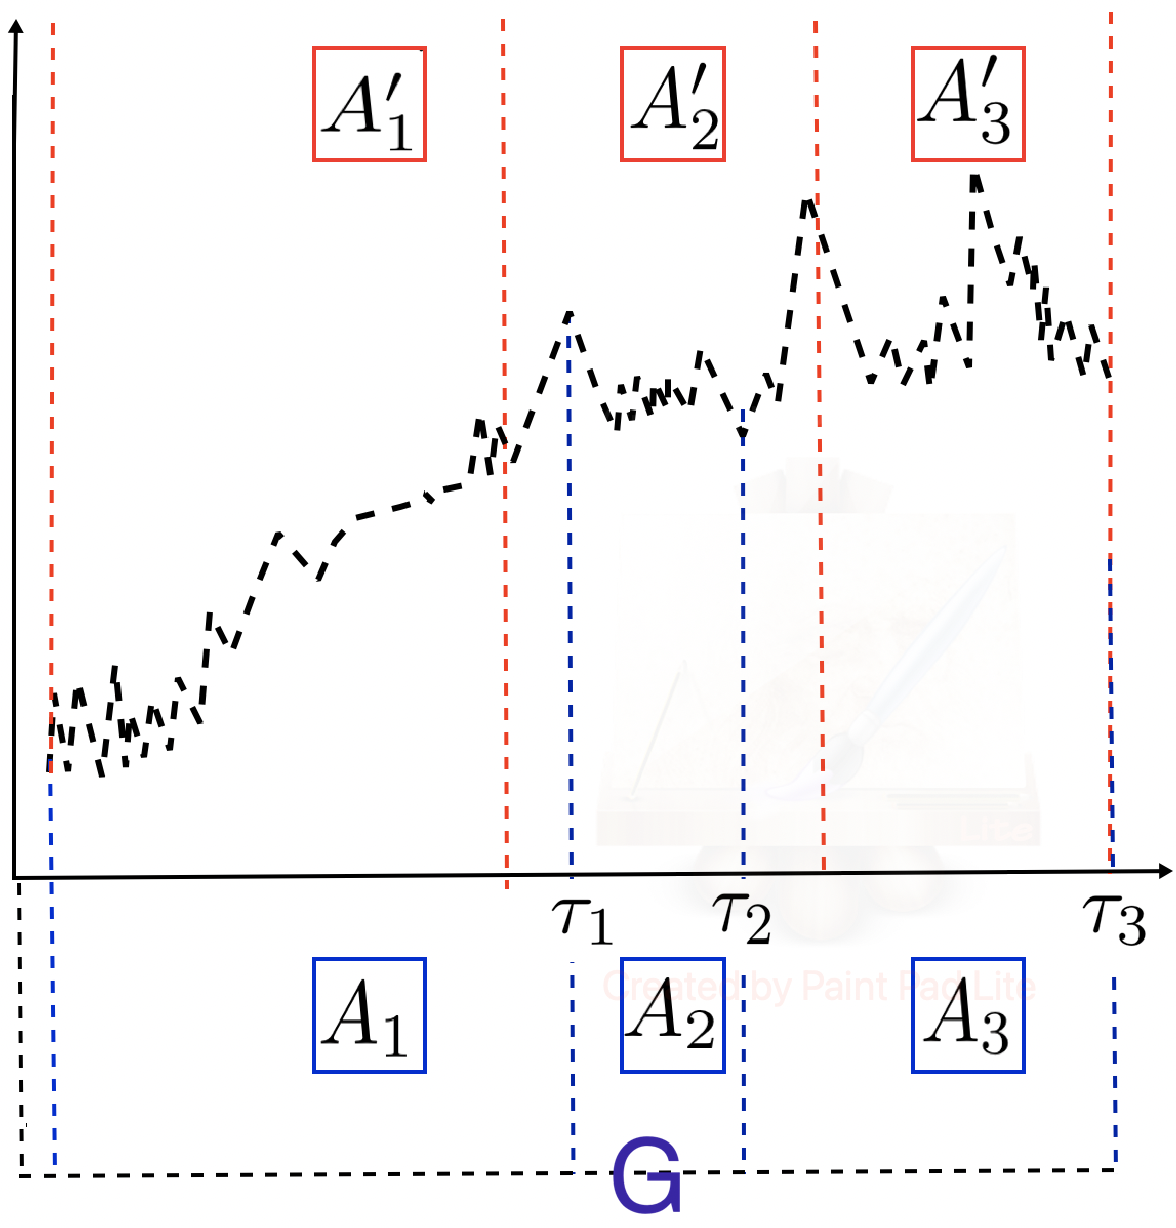
\includegraphics[width=400px,height=400px]{figure/cover} \caption{Kapsama Ölçütü}\label{fig:unnamed-chunk-1}
\end{figure}

Değişim noktası tespiti için metrikler, kümeleme metrikleri veya sınıflandırma metrikleri uyarlanarak kullanılabilir. Bu bölümde kümeleme analizinden uyarlanarak hesaplanan kapsama ölçütü (cover metric) tanıtılmıştır.

K işaretleyici sayısı \((k=1,...,K)\) olmak üzere, \(k.\) işaretleyici tarafından belirlenen değişim noktalarının konumları \(T_k = \{\tau_1,...,\tau_{n_k}\}\) ile gösterilir. \(\tau_i < \tau_j\) koşulunu sağlamak için \(i < j\) olmalıdır. \(T_k\), \([1, T]\) aralığını \(A_j\) adı verilen ayrık kümeler halinde bölen bir bölüm \(G_k\)'yi belirtir. Burada \(A_j\), \(j = 1,...,n_k +1\) için \(\tau_{j} -1\)'den \(\tau_{j} -1\)'e olan parçadır. Notasyon kolaylığı için \(\tau_0 = 1\) ve \(\tau_{n_k+1} = T +1\) kullanılır.

İki küme için \(A, A' \subseteq [1, T ]\) Jaccard indeksi, ayrıca iki kümenin kesişimi bölü birleşimi olarak da bilinir. \[J(A,A')=\frac{|A\cap A'|}{|A\cup A'|}\]

Kapsama metriğini \(G\) ve \(G'\) olarak tanımlarız.

\[C(G,G') = \frac{1}{T} \sum_{A \in G} |A| \cdot \max_{A' \in G'} J(A,A')\].

İşaretleyiciler tarafından sağlanan temel doğruluk bölümlerinin \(\{G_k\}_{k=1}^K\), bir algoritma tarafından verilen bir \(S\) bölümü için, \(C(G_k,S)\) ortalamasını hesaplayarak işaretleyicilerin tek bir performansını değerlendirilir.

\hypertarget{f1-puanux131}{%
\section{F1 Puanı}\label{f1-puanux131}}

Değişim noktası tespiti algoritmalarını değerlendirmeye ilişkin alternatif bir görüş, değişim noktası tespitini bir sınıflandırma problemi olarak kabul eder. Burada her bir gözlem ``değişim noktası'' veya ``tipik gözlem'' sınıflarına ait olarak değerlendirilir (Aminikhanghahi ve Cook, 2017; Killick, Fearnhead ve Eckley, 2012).

Değişim noktalarının sayısı genellikle serideki gözlem sayısından çok küçüktür. Bu nedenle doğruluk oranı gibi ölçütler oldukça çarpık olacaktır.

F puanında, bir algoritmanın performansı kesinlik (\(P\)) (doğru tespit edilen değişim noktalarının tespit edilen değişim noktalarının sayısına oranı) ve duyarlılık (doğru tespit edilen değişim noktalarının gerçek değişim noktalarının sayısına oranı) kullanılarak ölçülür (\(\beta = 1\) olarak varsayılır).

\[F_{\beta} = \frac{(1 + \beta^2) \cdot P \cdot R}{(\beta^2 \cdot P) + R}\]

\(X\), bir tespit algoritması ile bulunan değişim noktası konumları olsun. \(T^* = \cup T_k\), tüm işaretleyicilerin birleşik kümesidir. Değişim noktalarının gerçek konumları \(T\) için, algoritmalar ile elde edilen gerçek pozitifler \(TP(T, X)\) olarak tanımlanır (\(\tau \in T\)).Bu küme içindeki her bir \(\tau\), \(|\tau - x| \leq M\) koşulunu sağlayan en az bir \(x \in X\) için bulunur. Ancak bir \(\tau \in T\) için yalnızca bir \(x \in X\) kullanılır.

\begin{figure}
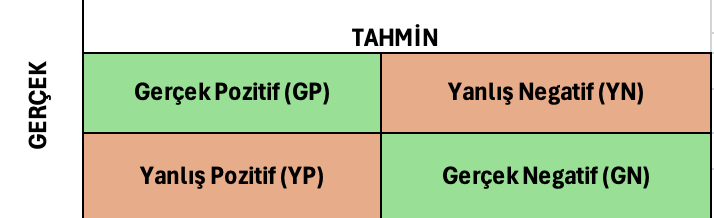
\includegraphics[width=357px,height=109px]{figure/conmat} \caption{Karışıklık matrisi}\label{fig:unnamed-chunk-2}
\end{figure}

\begin{itemize}
\tightlist
\item
  Gerçek Pozitif (GP): Doğru olarak tahmin edilen, gerçekte de doğru olan değerler,
\item
  Gerçek Negatif (GN): Yanlış olarak tahmin edilen, gerçekte de yanlış olan değerler,
\item
  Yanlış Pozitif (YP): Doğru olarak tahmin edilen, gerçekte yanlış olan değerler,
\item
  Yanlış Negatif (YN): Yanlış olarak tahmin edilen, gerçekte doğru olan değerleri ifade etmektedir.
\end{itemize}

\hypertarget{doux11fruluk-accuracy}{%
\subsubsection{Doğruluk (Accuracy)}\label{doux11fruluk-accuracy}}

Doğru tahmin edilen değerlerin, tüm değerlere bölünmesi ile elde edilmektedir. Doğruluk değeri, 0 ile 1 arasındadır. Doğruluk değeri 1'e yaklaştıkça başarı artmaktadır(Kelle ve Hüseyin, 2022).

\[Doğruluk = \frac{(GP + GN)}{(GP + GN + FP + FN)}\]

\hypertarget{duyarlux131lux131k-recall}{%
\subsubsection{Duyarlılık (Recall)}\label{duyarlux131lux131k-recall}}

Doğru olarak tahmin etmemiz gereken değerlerin, ne kadarını doğru tahmin ettiğimizi belirtmektedir. Duyarlılık değeri, gerçekte doğru olan ve doğru olarak tahmin edilen değerlerin, tüm doğru değerlere bölünmesi ile elde edilmektedir(Kelle ve Hüseyin, 2022).

\[Duyarlilik =  \frac{GP}{(GP + FN)}\]

\hypertarget{kesinlik-precision}{%
\subsubsection{Kesinlik (Precision)}\label{kesinlik-precision}}

Doğru olarak tahmin ettiğimiz değerlerin, ne kadarının gerçekte doğru olduğunu göstermektedir. Kesinlik değeri, gerçekte doğru olan ve doğru olarak tahmin edilen değerlerin, doğru olarak tahmin edilen tüm değerlere bölünmesi ile elde edilmektedir(Kelle ve Hüseyin, 2022).

\[Kesinlik =  \frac{GP}{(GP + FP)}\]

\hypertarget{f1-skoru-f1-score}{%
\subsubsection{F1 Skoru (F1 Score)}\label{f1-skoru-f1-score}}

F1 skoru, duyarlılık ve kesinlik değerlerinin harmonik ortalamasının hesaplanması ile elde edilmektedir. Her iki değerinde hesaplamaya katılarak dengeli bir değer elde edilmesi amaçlanmaktadır. Eşit dağılıma sahip olmayan veri setlerinde başarılı sonuçlar elde etmek için kullanılmaktadır(Kelle ve Hüseyin, 2022).

\[ F1 Skoru = \frac{2 * Kesinlik * Duyarlılık}{(Kesinlik + Duyarlılık)} \]

\hypertarget{Bolum3}{%
\chapter{Uygulama}\label{Bolum3}}

Uygulamada yirmi yapay veri ve onbir gerçek veri kullanılmıştır. Yapay verilerin her biri farklı sayıda değişim noktasına sahip olacak şekilde üretilmiştir. Gerçek veriler ise farklı alanlardan alınmıştır. Verilerin performanslarını belirlemek amacıyla F1 puanı ve kapsama ölçütü kullanılmıştır. Çalışmada R ve Python programlama dilleri kullanılmıştır. Uygulamada kullanılan veriler ve kodlar github sayfasında (\url{https://github.com/eyildiztepe/ChangePointDetection}) paylaşılmıştır.

\hypertarget{veri}{%
\section{Veri}\label{veri}}

Bu bölümde üretilen yapay veriler ve uygulamada kullanılan gerçek veriler hakkında bilgi verilmiştir.

\hypertarget{yapay-veri}{%
\subsection{Yapay Veri}\label{yapay-veri}}

Çalışmada kullanılan yapay veriler farklı sayıda değişim noktasına (DN) sahip olacak şekilde R programlama dili kullanılarak üretilmiştir. Yapay verilerin örneklem genişlikleri, ortalaması 2000, standart sapması 500 olan Normal dağılımndan, verideki değişim noktası sayısı ortalaması 2.8 olan Poisson dağılımından ve DN'lerin konumları ise Uniform dağılımından üretilmiştir. Kullanılan verilerin özellikleri Tablo \ref{tab:nvar1}'de verilmiştir.

\begin{longtable}[]{@{}llll@{}}
\caption{\label{tab:nvar1} Yapay Veriler}\tabularnewline
\toprule\noalign{}
Veri & Gözlem Sayısı & DN Sayısı & DN Konumu \\
\midrule\noalign{}
\endfirsthead
\toprule\noalign{}
Veri & Gözlem Sayısı & DN Sayısı & DN Konumu \\
\midrule\noalign{}
\endhead
\bottomrule\noalign{}
\endlastfoot
1 & 1687 & 4 & 516, 578 ,779,1499 \\
2 & 2092 & 3 & 564,1003,1347 \\
3 & 1582 & 4 & 175,553,1186,1347 \\
4 & 2798 & 3 & 951,985,2315 \\
5 & 2165 & 3 & 1034,1835,1892 \\
6 & 1590 & 4 & 631,698,1208,1481 \\
7 & 2244 & 1 & 1578 \\
8 & 2369 & 3 & 788,958,1768 \\
9 & 2288 & 4 & 316,493, 587,1606 \\
10 & 1847 & 4 & 153,300, 469,1172 \\
11 & 2756 & 3 & 2119,2168,2377 \\
12 & 2195 & 5 & 909,1004,1317,1422,1749 \\
13 & 1689 & 2 & 479,611 \\
14 & 893 & 2 & 552,837 \\
15 & 2562 & 1 & 575 \\
16 & 1978 & 1 & 293 \\
17 & 1992 & 2 & 955,1798 \\
18 & 2472 & 3 & 1470,1786,2365 \\
19 & 2411 & 3 & 393,874,1047 \\
20 & 2297 & 2 & 79,1622 \\
\end{longtable}

\hypertarget{geruxe7ek-veri}{%
\subsection{Gerçek Veri}\label{geruxe7ek-veri}}

Çalışmada farklı alanlardan gerçek veriler kullanılmıştır. Veriler (\url{https://github.com/alan-turing-institute/TCPD/tree/master/datasets}) adresinden temin edilmiştir. Gerçek verilerin özellikleri Tablo \ref{tab:ngercek}'de verilmiştir.

\begin{longtable}[]{@{}lllllll@{}}
\caption{\label{tab:ngercek} Gerçek Veriler}\tabularnewline
\toprule\noalign{}
Veri & GS & 1.DNS & 2.DNS & 3.DNS & 4.DNS & 5.DNS \\
\midrule\noalign{}
\endfirsthead
\toprule\noalign{}
Veri & GS & 1.DNS & 2.DNS & 3.DNS & 4.DNS & 5.DNS \\
\midrule\noalign{}
\endhead
\bottomrule\noalign{}
\endlastfoot
Bitcoin & NA & 4 & 1 & 1 & 7 & 7 \\
Brent-spot. & 500 & 3 & 2 & 5 & 9 & 11 \\
Children-per women & 301 & 2 & 1 & 2 & 4 & 2 \\
Co2- canada & 215 & 2 & 6 & 2 & 5 & 7 \\
Debt -Ireland & 21 & 2 & 2 & 2 & 4 & 2 \\
Rail-lines & 37 & 2 & 2 & 2 & 2 & 1 \\
Rather-stock & 600 & 1 & 2 & 1 & 2 & 2 \\
Scanline-42049 & 481 & 10 & 7 & 2 & 7 & 7 \\
Shangai-license & 205 & 1 & 1 & 1 & 1 & 2 \\
Usd-isk & 247 & 2 & 4 & 1 & 3 & 2 \\
Well-log & 675 & 11 & 9 & 9 & 2 & 17 \\
\end{longtable}

\emph{GS: Gözlem sayısı ,DNS: Değişim Noktası Sayısı}

Çalışmada kullanılan gerçek veriler 5 ayrı işaretleyici tarafından işaretlenmiştir (Van den Burg ve Williams, 2020).Bu nedenle değişim noktası konumları değişiklik göstermektedir .

\hypertarget{deux11fiux15fim-noktasux131-analizi}{%
\section{Değişim Noktası Analizi}\label{deux11fiux15fim-noktasux131-analizi}}

Bu bölümde kullanılan yöntemler ile elde edilen sonuçlara yer verilmiştir. Kullanılan fonksiyonların varsayılan ayarları ile elde edilen sonuçlar F1 puanı varsayılan ve kapsama ölçütü varsayılan olarak adlandırılmıştır. Ayrıca, argümanların değerleri değiştirilerek elde edilen en iyi sonuçlar F1 puanı ayarlanmış ve kapsama ölçütü ayarlanmış olarak sunulmuştur.

\hypertarget{yapay-veriler-iuxe7in-sonuuxe7lar}{%
\subsection{Yapay Veriler için Sonuçlar}\label{yapay-veriler-iuxe7in-sonuuxe7lar}}

Bu bölümde yapay veriler için elde edilen sonuçlara yer verilmiştir.

\begin{longtable}[]{@{}llllll@{}}
\caption{\label{tab:nvar8} F1 puanı (Varsayılan)}\tabularnewline
\toprule\noalign{}
Veri & AMOC & BINSEG & SEGMENTED & PROPHET & PELT \\
\midrule\noalign{}
\endfirsthead
\toprule\noalign{}
Veri & AMOC & BINSEG & SEGMENTED & PROPHET & PELT \\
\midrule\noalign{}
\endhead
\bottomrule\noalign{}
\endlastfoot
1 & 0,5714 & 0,9091 & 0,2857 & 0,2857 & 0,4000 \\
2 & 0,6667 & 0,4000 & 0,3333 & 0,1818 & 0,4444 \\
3 & 0,5714 & 0,9091 & 0,1290 & 0,2000 & 0,4000 \\
4 & 0,6667 & 0,8000 & 0,3333 & 0,2222 & 0,7500 \\
5 & 0,6667 & 0,6000 & 0,4444 & 0,2500 & 0,6666 \\
6 & 0,5714 & 0,5455 & 0,4000 & 0,1538 & 0,4000 \\
7 & 0,5000 & 0,2500 & 0,5000 & 0,3333 & 0,5000 \\
8 & 0,6667 & 0,8000 & 0,5000 & 0,2222 & 0,6000 \\
9 & 0,2857 & 0,5455 & 0,4000 & 0,1818 & 0,3636 \\
10 & 0,5714 & 0,7273 & 0,6000 & 0,1666 & 0,4615 \\
11 & 0,6667 & 0,6000 & 0,5000 & 0,2222 & 0,4444 \\
12 & 0,5000 & 0,8333 & 0,1666 & 0,1666 & 0,5000 \\
13 & 0,8000 & 0,6667 & 0,6666 & 0,2857 & 0,5714 \\
14 & 0,8000 & 0,6667 & 0,6666 & 0,2857 & 0,5714 \\
15 & 0,9998 & 0,5000 & 0,5000 & 0,4000 & 0,4000 \\
16 & 0,9999 & 0,5000 & 0,5000 & 0,4000 & 0,4000 \\
17 & 0,8000 & 0,6667 & 0,6666 & 0,2857 & 0,5714 \\
18 & 0,6667 & 0,8000 & 0,5000 & 0,2222 & 0,4000 \\
19 & 0,6667 & 0,8000 & 0,5000 & 0,2222 & 0,4444 \\
20 & 0,8000 & 0,4444 & 0,3333 & 0,2857 & 0,2857 \\
\end{longtable}

Algoritmalar varsayılan parametre ayarlarıyla çalıştırıldığında (\ref{tab:nvar8}), yirmi yapay verinin sekizinde BinSeg, altısında AMOC ve birinde PELT 0,7 ve üzerinde F1 puanına sahipken, parçalı regresyon ve Prophet algoritmasında F1 puanı 0,7 ve üzerinde olan veri bulunmamaktadır.
Varsayılan parametrelerle çalıştırılan algoritmalardan Prophet on yedi, parçalı regresyon üç, AMOC, BinSeg ve Pelt algoritmalarında birer tane 0,3'ün altında F1 puanına sahip veri bulunmaktadır.

\begin{longtable}[]{@{}llllll@{}}
\caption{\label{tab:nvar9} Kapsama Ölçütü (Varsayılan)}\tabularnewline
\toprule\noalign{}
Veri & AMOC & BINSEG & SEGMENTED & PROPHET & PELT \\
\midrule\noalign{}
\endfirsthead
\toprule\noalign{}
Veri & AMOC & BINSEG & SEGMENTED & PROPHET & PELT \\
\midrule\noalign{}
\endhead
\bottomrule\noalign{}
\endlastfoot
1 & 0,5975 & 0,9895 & 0,3740 & 0,3607 & 0,6843 \\
2 & 0,5388 & 0,8881 & 0,5185 & 0,5600 & 0,7686 \\
3 & 0,4937 & 0,9943 & 0,2397 & 0,5151 & 0,7953 \\
4 & 0,5850 & 0,8989 & 0,4876 & 0,5495 & 0,8897 \\
5 & 0,7707 & 0,9687 & 0,8126 & 0,6164 & 0,7706 \\
6 & 0,6079 & 0,8822 & 0,7007 & 0,3625 & 0,5339 \\
7 & 0,9648 & 0,7995 & 0,7807 & 0,4670 & 0,8523 \\
8 & 0,6084 & 0,8848 & 0,6725 & 0,6173 & 0,7047 \\
9 & 0,6629 & 0,9467 & 0,4937 & 0,5129 & 0,6060 \\
10 & 0,6269 & 0,9288 & 0,7368 & 0,4726 & 0,4510 \\
11 & 0,8764 & 0,9464 & 0,8185 & 0,9991 & 0,6856 \\
12 & 0,5639 & 0,8220 & 0,6032 & 0,6158 & 0,5461 \\
13 & 0,8771 & 0,7478 & 0,8771 & 0,5563 & 0,4660 \\
14 & 0,8932 & 0,9567 & 0,8911 & 0,4304 & 0,7085 \\
15 & 0,9992 & 0,9863 & 0,8634 & 0,5091 & 0,4972 \\
16 & 0,9950 & 0,7715 & 0,8828 & 0,4541 & 0,4058 \\
17 & 0,8408 & 0,8620 & 0,8403 & 0,5809 & 0,5871 \\
18 & 0,7744 & 0,9956 & 0,8502 & 0,4184 & 0,4871 \\
19 & 0,6932 & 0,9925 & 0,7623 & 0,4422 & 0,4285 \\
20 & 0,5905 & 0,7208 & 0,4578 & 0,4711 & 0,5644 \\
\end{longtable}

Tablo \ref{tab:nvar9}'daki sonuçlara göre, BinSeg varsayılan parametre ayarlarıyla çalıştırıldığında tüm verilerde 0,7'nin üzerinde kapsama ölçütü değerine sahiptir. Parçalı regresyon on ikisinde, AMOC dokuzunda, Pelt yedisinde ve Prophet birinde 0,7 ve üzerinde kapsama ölçütü değerine sahip olduğu görülmektedir.

Varsayılan ayarlar çalıştırılan algoritmalardan sadece parçalı regresyonda bir veri 0,3'ün altında kapsama ölçütü değerine sahiptir.

\begin{longtable}[]{@{}llllll@{}}
\caption{\label{tab:nvar10} F1 Puanı (Ayarlanmış)}\tabularnewline
\toprule\noalign{}
Veri & AMOC & BINSEG & SEGMENTED & PROPHET & PELT \\
\midrule\noalign{}
\endfirsthead
\toprule\noalign{}
Veri & AMOC & BINSEG & SEGMENTED & PROPHET & PELT \\
\midrule\noalign{}
\endhead
\bottomrule\noalign{}
\endlastfoot
1 & 0,5714 & 0,9997 & 0,4444 & 0,2500 & 0,6000 \\
2 & 0,6667 & 0,5000 & 0,5000 & 0,4000 & 0,5000 \\
3 & 0,5714 & 0,9994 & 0,4000 & 0,2500 & 0,4000 \\
4 & 0,6667 & 0,9996 & 0,4000 & 0,2500 & 0,7500 \\
5 & 0,6667 & 0,7500 & 0,4000 & 0,2857 & 0,6666 \\
6 & 0,5714 & 0,6000 & 0,4000 & 0,3333 & 0,2857 \\
7 & 0,5000 & 0,5000 & 0,5000 & 0,4000 & 0,5000 \\
8 & 0,6667 & 0,7500 & 0,5000 & 0,2500 & 0,5454 \\
9 & 0,2857 & 0,6000 & 0,4000 & 0,2222 & 0,3636 \\
10 & 0,5714 & 0,8000 & 0,6000 & 0,2000 & 0,6000 \\
11 & 0,6667 & 0,7500 & 0,5000 & 0,2500 & 0,5714 \\
12 & 0,5000 & 0,8333 & 0,1666 & 0,3636 & 0,5000 \\
13 & 0,8000 & 0,9987 & 0,6666 & 0,3333 & 0,6666 \\
14 & 0,8000 & 0,6667 & 0,6666 & 0,3333 & 0,6666 \\
15 & 0,9998 & 0,9989 & 0,5000 & 0,5000 & 0,5000 \\
16 & 0,9999 & 0,9967 & 0,5000 & 0,5000 & 0,5000 \\
17 & 0,8000 & 0,9985 & 0,6666 & 0,3333 & 0,6666 \\
18 & 0,6667 & 0,9978 & 0,5000 & 0,2500 & 0,5000 \\
19 & 0,6667 & 0,9949 & 0,5000 & 0,2500 & 0,5000 \\
20 & 0,8000 & 0,6667 & 0,3333 & 0,3333 & 0,3333 \\
\end{longtable}

Ayarlanmış parametreler sonucunda en iyi F1 puanı değerleri BinSeg ile elde edilmiştir. Prophet ve parçalı regresyon algoritmalarında hiç bir veri 0,7 ve üzerinde F1 puanına sahip değildir. Pelt algoritmasında bir tane verinin 0,7'nin üzerinde olduğu görülmektedir.

Prophet algoritmasının en kötü F1 puanı değerlerini verdiği görülmektedir. AMOC, parçalı regresyon ve Pelt algoritmalarında 0,3 'ün altında birer tane veri bulunmaktadır.

\begin{longtable}[]{@{}llllll@{}}
\caption{\label{tab:nvar11} Kapsama Ölçütü (Ayarlanmış)}\tabularnewline
\toprule\noalign{}
Veri & AMOC & BINSEG & SEGMENTED & PROPHET & PELT \\
\midrule\noalign{}
\endfirsthead
\toprule\noalign{}
Veri & AMOC & BINSEG & SEGMENTED & PROPHET & PELT \\
\midrule\noalign{}
\endhead
\bottomrule\noalign{}
\endlastfoot
1 & 0,5975 & 0,9930 & 0,9930 & 0,6104 & 0,7081 \\
2 & 0,5388 & 0,8914 & 0,8914 & 0,6793 & 0,8194 \\
3 & 0,4937 & 0,9950 & 0,9950 & 0,6152 & 0,9246 \\
4 & 0,5850 & 0,9957 & 0,9957 & 0,6830 & 0,8840 \\
5 & 0,7707 & 0,9688 & 0,9688 & 0,7494 & 0,7706 \\
6 & 0,6079 & 0,8853 & 0,8853 & 0,3967 & 0,5599 \\
7 & 0,9648 & 0,9648 & 0,9648 & 0,6002 & 0,9670 \\
8 & 0,6084 & 0,8831 & 0,8831 & 0,6700 & 0,7364 \\
9 & 0,6629 & 0,9467 & 0,9467 & 0,5665 & 0,6067 \\
10 & 0,6269 & 0,9092 & 0,9092 & 0,4866 & 0,7201 \\
11 & 0,8764 & 0,9689 & 0,9689 & 0,9998 & 0,9387 \\
12 & 0,5639 & 0,8220 & 0,8220 & 0,6338 & 0,5604 \\
13 & 0,8771 & 0,9976 & 0,9976 & 0,6158 & 0,6509 \\
14 & 0,8932 & 0,9567 & 0,9567 & 0,5356 & 0,8589 \\
15 & 0,9992 & 0,9992 & 0,9992 & 0,5255 & 0,8189 \\
16 & 0,9950 & 0,9950 & 0,9950 & 0,5825 & 0,7296 \\
17 & 0,8408 & 0,9980 & 0,9980 & 0,7171 & 0,7905 \\
18 & 0,7744 & 0,9976 & 0,9976 & 0,4701 & 0,6171 \\
19 & 0,6932 & 0,9983 & 0,9983 & 0,4816 & 0,6680 \\
20 & 0,5905 & 0,9854 & 0,9854 & 0,5511 & 0,7184 \\
\end{longtable}

Ayarlanan parametreler ile hesaplanan kapsama ölçütü değerinin BinSeg ve parçalı regresyon algoritmalarının tamamında 0,8'in üzerinde olduğu görülmektedir. Pelt için on dört, AMOC için dokuz ve Prophet algortiması için üç verinin 0,7'nin üzerindekapsama ölçütü değerine sahip olduğu görülmektedir.
Ayarlanan parametrelerle çalıştırılan beş farklı algoritmanın kullanıldığı yirmi verinin hiçbirinde 0,3'ün altından kapsama ölçütü değeri bulunmamaktadır.

\hypertarget{geruxe7ek-veriler-iuxe7in-sonuuxe7lar}{%
\subsection{Gerçek Veriler için Sonuçlar}\label{geruxe7ek-veriler-iuxe7in-sonuuxe7lar}}

Bu bölümde gerçek veriler için elde edilen sonuçlara yer verilmiştir.

\begin{longtable}[]{@{}llllll@{}}
\caption{\label{tab:nvar2} F1 puanı (Varsayılan)}\tabularnewline
\toprule\noalign{}
Veri & AMOC & BINSEG & PELT & SEGMENTED & PROPHET \\
\midrule\noalign{}
\endfirsthead
\toprule\noalign{}
Veri & AMOC & BINSEG & PELT & SEGMENTED & PROPHET \\
\midrule\noalign{}
\endhead
\bottomrule\noalign{}
\endlastfoot
Bitcoin & 0,3670 & 0,4897 & 0,2663 & 0,3670 & 0,2341 \\
Brent-spot & 0,2718 & 0,6431 & 0,4244 & 0,6590 & 0,3904 \\
Children-per women & 0,6175 & 0,5902 & 0,3366 & 0,8440 & 0,5168 \\
Co2- canada & 0,5441 & 0,8194 & 0,8194 & 0,3938 & 0,6315 \\
Debt -Ireland & 0,7603 & 1,0000 & 0,7603 & 0,7603 & 0,6086 \\
Rail-lines & 0,8462 & 0,8000 & 0,4690 & 1,0000 & 0,2666 \\
Rather-stock & 0,2718 & 0,3392 & 0,4710 & 0,4886 & 0,5292 \\
Scanline-42049 & 0,4926 & 0,7400 & 0,5151 & 0,2463 & 0,3902 \\
Shangai-license & 0,8679 & 0,6511 & 0,6666 & 0,6495 & 0,5316 \\
Usd-isk & 0,7854 & 0,6093 & NA & 0,7881 & 0,5956 \\
Well-log & NA & 0,7289 & 0,4235 & 0,6912 & 0,3589 \\
\end{longtable}

Varsayılan parametre ayarlarıyla algoritmalar çalıştırıldığında, on bir verinin beşinde BinSeg, dördünde AMOC ve parçalı regresyon, ikisinde PELT 0,7 ve üzerinde F1 puanına sahipken Prophet algoritmasında F1 puanı 0,7 ve üzerinde olan veri bulunmamaktadır.

Varsayılan ayarlarda, on bir verinin ikisinde AMOC ve Prophet ile, birinde PELT ve parçalı regresyon ile 0,3'ün altında F1 puanı elde edilmiştir.

BinSeg algoritmasında F1 puanı 0,3 ve altında olan veri bulunmamaktadır.
Değişim noktası tespit edilemeyen durumlar (NA) ile gösterilmiştir.

\begin{longtable}[]{@{}llllll@{}}
\caption{\label{tab:nvar3} Kapsama Ölçütü (Varsayılan)}\tabularnewline
\toprule\noalign{}
Veri & AMOC & BINSEG & PELT & SEGMENTED & PROPHET \\
\midrule\noalign{}
\endfirsthead
\toprule\noalign{}
Veri & AMOC & BINSEG & PELT & SEGMENTED & PROPHET \\
\midrule\noalign{}
\endhead
\bottomrule\noalign{}
\endlastfoot
Bitcoin & 0,7640 & 0,7354 & 0,3022 & 0,5322 & 0,1941 \\
Brent-spot & 0,4251 & 0,5921 & 0,4535 & 0,4945 & 0,2992 \\
Children-per women & 0,7838 & 0,7663 & 0,7721 & 0,6282 & 0,2753 \\
Co2- canada & 0,5264 & 0,7291 & 0,7393 & 0,5135 & 0,3409 \\
Debt -Ireland & 0,5844 & 0,6607 & 0,5446 & 0,5861 & 0,4000 \\
Rail-lines & 0,7682 & 0,7732 & 0,4408 & 0,7890 & 0,3081 \\
Rather-stock & 0,3870 & 0,3923 & 0,3970 & 0,5164 & 0,3470 \\
Scanline-42049 & 0,4305 & 0,7502 & 0,4157 & 0,3859 & 0,3249 \\
Shangai-license & 0,9105 & 0,7691 & 0,3132 & 0,8272 & 0,2458 \\
Usd-isk & 0,8577 & NA & NA & 0,5248 & 0,2752 \\
Well-log & 0,4527 & 0,7696 & 0,4285 & 0,4146 & 0,3743 \\
\end{longtable}

Varsayılan ayarlar ile, on bir verinin yedisinde BinSeg, beşinde AMOC, ikisinde PELT ve parçalı regresyon ile 0,7 ve üzerinde kapsama ölçütü değerleri elde edilmiştir.

Prophet algoritmasında hiçbir veri için kapsama ölçütü değeri 0,7 nin üzerinde değildir.
Varsayılan ayarlar ile Prophet algoritmasında başarılı kapsama ölçütü değerleri elde edilemediği görülmektedir. Prophet on bir verinin beşinde 0,3 ve altında kapsama ölçütü değerine sahiptir.
Değişim noktası tespit edilemeyen durumlar (NA) ile gösterilmiştir.

\begin{longtable}[]{@{}llllll@{}}
\caption{\label{tab:nvar4} F1 Puanı (Ayarlanmış)}\tabularnewline
\toprule\noalign{}
Veri & AMOC & BINSEG & PELT & SEGMENTED & PROPHET \\
\midrule\noalign{}
\endfirsthead
\toprule\noalign{}
Veri & AMOC & BINSEG & PELT & SEGMENTED & PROPHET \\
\midrule\noalign{}
\endhead
\bottomrule\noalign{}
\endlastfoot
Bitcoin & 0,3670 & 0,6124 & 0,3940 & 0,4523 & 0,2743 \\
Brent-spot & 0,2718 & 0,6341 & 0,4481 & 0,6590 & 0,3704 \\
Children-per women & 0,6175 & 0,5902 & 0,6388 & 0,8440 & 0,5168 \\
Co2- canada & 0,5441 & 0,8776 & 0,3595 & 0,7142 & 0,6045 \\
Debt -Ireland & 0,7603 & 0,9583 & 0,9583 & 0,9795 & 0,9795 \\
Rail-lines & 0,8461 & 0,8316 & 0,7234 & 0,9655 & 0,9655 \\
Rather-stock & 0,2718 & 0,3728 & 0,5316 & 0,4243 & 0,5292 \\
Scanline-42049 & 0,4926 & 0,8331 & 0,5704 & 0,8648 & 0,4581 \\
Shangai-license & 0,8679 & 0,6511 & 0,2025 & 0,6495 & 0,5316 \\
Usd-isk & 0,7854 & 0,6093 & 0,6007 & 0,7881 & 0,5956 \\
Well-log & 0,2791 & 0,7289 & 0,5760 & 0,6912 & 0,3589 \\
\end{longtable}

Ayarlanmış parametreler ile en iyi F1 puanı değerleri parçalı regresyon ile alınmıştır. On bir veri setinin altısında parçalı regresyon, beşinde BinSeg, dördünde AMOC, ikisinde PELT ve Prophet'in 0,7 ve üzerinde F1 puanına sahip olduğu görülmektedir.

Tablo \ref{tab:nvar4}'e göre parçalı regresyon ve BinSeg algoritmaları denenen tüm gerçek veriler için 0,3 ve üzerinde F1 puanı elde etmişlerdir. Ancak AMOC algoritması için F1 puanı onbir verinin üçünde 0,3'ün altındadır.

\begin{longtable}[]{@{}llllll@{}}
\caption{\label{tab:nvar5} Kapsama Ölçütü (Ayarlanmış)}\tabularnewline
\toprule\noalign{}
Veri & AMOC & BINSEG & PELT & SEGMENTED & PROPHET \\
\midrule\noalign{}
\endfirsthead
\toprule\noalign{}
Veri & AMOC & BINSEG & PELT & SEGMENTED & PROPHET \\
\midrule\noalign{}
\endhead
\bottomrule\noalign{}
\endlastfoot
Bitcoin & 0,7640 & 0,4352 & 0,2182 & 0,3833 & 0,2045 \\
Brent-spot & 0,4251 & 0,4858 & 0,3257 & 0,5273 & 0,3206 \\
Children-per women & 0,7938 & 0,7625 & 0,7635 & 0,7062 & 0,3485 \\
Co2- canada & 0,5264 & 0,7001 & 0,7494 & 0,6622 & 0,4366 \\
Debt -Ireland & 0,5844 & 0,8136 & 0,7042 & 0,8217 & 0,6919 \\
Rail-lines & 0,7665 & 0,7731 & 0,5113 & 0,6964 & 0,6222 \\
Rather-stock & 0,3870 & 0,3941 & 0,4840 & 0,4488 & 0,3470 \\
Scanline-42049 & 0,4305 & 0,8570 & 0,4157 & 0,7944 & 0,4097 \\
Shangai-license & 0,9105 & 0,7961 & 0,3955 & 0,8058 & 0,3625 \\
Usd-isk & 0,8577 & 0,7549 & 0,5609 & 0,7819 & 0,4211 \\
Well-log & 0,4527 & 0,6371 & 0,4873 & 0,5511 & 0,4615 \\
\end{longtable}

Ayarlanmış parametreler ile algoritmalar çalıştırıldığında, kapsama ölçütüne göre en iyi sonuçları BinSeg algoritması vermiştir. Denenen on bir verinin yedisinde BinSeg, beşinde AMOC ve parçalı regresyon, üçünde PELT 0,7 ve üzerinde kapsama metriğine sahipken Prophet algoritmasında kapsama metriği 0,7 ve üzerinde olan veri bulunmamaktadır.

Çalışmada incelenen algoritmaların ihtiyaç duyduğu parametre değerleri verilere göre en uygun hale getirildiğinde BinSeg ve parçalı regresyon algoritmalarının diğerlerine göre değişim noktalarının konumlarını belirlemede daha başarılı olduğu görülmüştür.

\hypertarget{kademeli-egzersiz-testi-verileri}{%
\section{Kademeli Egzersiz Testi Verileri}\label{kademeli-egzersiz-testi-verileri}}

Bu bölümde 15 sporcunun kademeli bir rampa testi sonucunda elde edilen veriler kullanılarak eşik egzersiz şiddetlerini değişim noktası belirleme yöntemleri ile tespit etmek denenmiştir.

\begin{longtable}[]{@{}llll@{}}
\caption{\label{tab:nvar6} Kapsama Ölçütü (Ayarlanmış)}\tabularnewline
\toprule\noalign{}
Veri & BINSEG & SEGMENTED & PELT \\
\midrule\noalign{}
\endfirsthead
\toprule\noalign{}
Veri & BINSEG & SEGMENTED & PELT \\
\midrule\noalign{}
\endhead
\bottomrule\noalign{}
\endlastfoot
1 & 0,7023 & 0,6688 & 0,7340 \\
2 & NA & 0,8232 & NA \\
3 & NA & 0,5097 & NA \\
4 & 0,7485 & 0,9547 & 0,7308 \\
5 & 0,9326 & 0,8972 & 0,7314 \\
6 & NA & 0,7793 & NA \\
7 & NA & 0,9493 & NA \\
8 & 1,0000 & 0,8930 & 0,8425 \\
9 & 0,8181 & 0,9545 & 0,8723 \\
10 & 0,8039 & 0,6843 & 0,7189 \\
11 & 1,0000 & 0,6111 & 0,5965 \\
12 & 1,0000 & 0,7270 & 0,9353 \\
13 & 0,6520 & 0,8486 & 0,9805 \\
14 & 0,5434 & 0,7423 & 1,0000 \\
15 & 0,7141 & 0,4571 & 0,8194 \\
\end{longtable}

Ayarlanan parametreler ile hesaplanan kapsama ölçütü değerinin parçalı regresyon algoritmasında yedi, Pelt ve BinSeg algoritmalarında ise altı veride 0,8'in üzerinde olduğu görülmektedir.
Ayarlanan parametrelerle çalıştırılan üç farklı algoritmanın kullanıldığı on beş verinin hiçbirinde 0,3'ün altından kapsama ölçütü değeri bulunmamaktadır.

İki değişim noktası tespit edilemeyen durumlar (NA) ile gösterilmiştir.

\begin{longtable}[]{@{}llll@{}}
\caption{\label{tab:nvar7} F1 Puanı (Ayarlanmış)}\tabularnewline
\toprule\noalign{}
Veri & BINSEG & SEGMENTED & PELT \\
\midrule\noalign{}
\endfirsthead
\toprule\noalign{}
Veri & BINSEG & SEGMENTED & PELT \\
\midrule\noalign{}
\endhead
\bottomrule\noalign{}
\endlastfoot
1 & 0,6600 & 0,6600 & 0,6600 \\
2 & NA & 1,0000 & NA \\
3 & NA & 0,6600 & NA \\
4 & 1,0000 & 1,0000 & 1,0000 \\
5 & 1,0000 & 1,0000 & 1,0000 \\
6 & NA & 1,0000 & NA \\
7 & NA & 1,0000 & NA \\
8 & 1,0000 & 1,0000 & 1,0000 \\
9 & 0,8571 & 0,8571 & 1,0000 \\
10 & 1,0000 & 1,0000 & 1,0000 \\
11 & 0,7499 & 0,8571 & 0,8571 \\
12 & 1,0000 & 1,0000 & 1,0000 \\
13 & 0,5714 & 0,8571 & 1,0000 \\
14 & 0,2857 & 0,8571 & 1,0000 \\
15 & 0,2857 & 0,4615 & 0,6600 \\
\end{longtable}

Ayarlanmış parametreler sonucunda en iyi F1 puanı değerleri parçalı regresyon ile elde edilmiştir. Parçalı regresyon algoritmasında on iki veri 0,8 ve üzerinde F1 puanına sahiptir. Pelt algoritmasında dokuz, BinSeg algoritmasında ise altı verinin 0,8'in üzerinde F1 puanına sahip olduğu görülmektedir.

Pelt ve parçalı regresyon algoritmalarının 0,3'ün altında F1 puanı yokken, BinSeg algoritmasında ise iki veride 0,3'ün altında F1 puanı elde edilmiştir.

İki değişim noktası tespit edilemeyen durumlar (NA) ile gösterilmiştir.

\hypertarget{Bolum4}{%
\chapter{Bölüm Başlığı}\label{Bolum4}}

\hypertarget{bu-bir-alt-baux15flux131k}{%
\section{Bu bir alt başlık}\label{bu-bir-alt-baux15flux131k}}

Bu bölümde şu konular yer almaktadır\ldots{}

\hypertarget{bu-ikinci-seviye-bir-alt-baux15flux131k}{%
\subsection{Bu ikinci seviye bir alt başlık}\label{bu-ikinci-seviye-bir-alt-baux15flux131k}}

\hypertarget{Bolum5}{%
\chapter{Bölüm 4 Başlık}\label{Bolum5}}

\hypertarget{bu-bir-alt-baux15flux131k-1}{%
\section{Bu bir alt başlık}\label{bu-bir-alt-baux15flux131k-1}}

Bu bölümde şu konular yer almaktadır\ldots{}

\hypertarget{bu-ikinci-seviye-bir-alt-baux15flux131k-1}{%
\subsection{Bu ikinci seviye bir alt başlık}\label{bu-ikinci-seviye-bir-alt-baux15flux131k-1}}

\hypertarget{sonuuxe7}{%
\chapter*{Sonuç}\label{sonuuxe7}}
\addcontentsline{toc}{chapter}{Sonuç}

If we don't want Conclusion to have a chapter number next to it, we can add the \texttt{\{-\}} attribute.

\textbf{More info}

And here's some other random info: the first paragraph after a chapter title or section head \emph{shouldn't be} indented, because indents are to tell the reader that you're starting a new paragraph. Since that's obvious after a chapter or section title, proper typesetting doesn't add an indent there.

\hypertarget{kaynaklar}{%
\chapter*{Kaynaklar}\label{kaynaklar}}
\addcontentsline{toc}{chapter}{Kaynaklar}

\markboth{Kaynaklar}{Kaynaklar}

\hypertarget{refs}{}
\begin{CSLReferences}{1}{0}
\leavevmode\vadjust pre{\hypertarget{ref-aminikhanghahi2017survey}{}}%
Aminikhanghahi, S. ve Cook, D. J. (2017). A survey of methods for time series change point detection. \emph{Knowledge and information systems}, \emph{51}(2), 339-367.

\leavevmode\vadjust pre{\hypertarget{ref-angel2000}{}}%
Angel, E. (2000). \emph{Interactive Computer Graphics : A Top-Down Approach with OpenGL}. Boston, MA: Addison Wesley Longman.

\leavevmode\vadjust pre{\hypertarget{ref-angel2001a}{}}%
Angel, E. (2001a). \emph{Batch-file Computer Graphics : A Bottom-Up Approach with QuickTime}. Boston, MA: Wesley Addison Longman.

\leavevmode\vadjust pre{\hypertarget{ref-angel2001b}{}}%
Angel, E. (2001b). \emph{test second book by angel}. Boston, MA: Wesley Addison Longman.

\leavevmode\vadjust pre{\hypertarget{ref-birge2007}{}}%
Birgé, L. ve Massart, P. (2007). Minimal penalties for Gaussian model selection. \emph{Probability theory and related fields}, \emph{138}, 33-73.

\leavevmode\vadjust pre{\hypertarget{ref-chen2000}{}}%
Chen, J., Gupta, A. K. ve Gupta, A. (2000). \emph{Parametric statistical change point analysis} (C. 192). Springer.

\leavevmode\vadjust pre{\hypertarget{ref-deussen2000}{}}%
Deussen, O. ve Strothotte, T. (2000). Computer-Generated Pen-and-Ink Illustration of Trees. \emph{{``Proceedings of''} SIGGRAPH 2000}, Computer Graphics Proceedings, Annual Conference Series, 13-18.

\leavevmode\vadjust pre{\hypertarget{ref-hipr1997}{}}%
Fisher, R., Perkins, S., Walker, A. ve Wolfart, E. (1997). \emph{Hypermedia Image Processing Reference}. New York, NY: John Wiley \& Sons.

\leavevmode\vadjust pre{\hypertarget{ref-goochandgooch2001}{}}%
Gooch, B. ve Gooch, A. (2001a). \emph{{Non-Photorealistic Rendering}}. Natick, Massachusetts: A K Peters.

\leavevmode\vadjust pre{\hypertarget{ref-goochandgooch2001a}{}}%
Gooch, B. ve Gooch, A. (2001b). \emph{Test second book by gooches}. Natick, Massachusetts: A K Peters.

\leavevmode\vadjust pre{\hypertarget{ref-guyon1999}{}}%
Guyon, X. ve Yao, J. (1999). On the underfitting and overfitting sets of models chosen by order selection criteria. \emph{Journal of Multivariate Analysis}, \emph{70}(2), 221-249.

\leavevmode\vadjust pre{\hypertarget{ref-hertzmann2000}{}}%
Hertzmann, A. ve Zorin, D. (2000). Illustrating Smooth Surfaces. \emph{Proceedings of SIGGRAPH 2000}, Computer Graphics Proceedings, Annual Conference Series, \emph{5}(17), 517-526.

\leavevmode\vadjust pre{\hypertarget{ref-hinkley1970}{}}%
Hinkley, D. V. (1970). Inference about the change-point in a sequence of random variables.

\leavevmode\vadjust pre{\hypertarget{ref-jain1989}{}}%
Jain, A. K. (1989). \emph{Fundamentals of Digital Image Processing}. Englewood Cliffs, New Jersey: Prentice-Hall.

\leavevmode\vadjust pre{\hypertarget{ref-jengupta1987}{}}%
Jen, T. ve Gupta, A. K. (1987). On testing homogeneity of variances for Gaussian models. \emph{Journal of Statistical Computation and Simulation}, \emph{27}(2), 155-173.

\leavevmode\vadjust pre{\hypertarget{ref-kelle2022mqtt}{}}%
Kelle, A. C. ve Hüseyin, Y. (2022). MQTT Trafi{ğ}inde DoS Sald{ı}r{ı}lar{ı}n{ı}n Makine {Ö}{ğ}renmesi ile S{ı}n{ı}fland{ı}r{ı}lmas{ı} ve Modelin SHAP ile Yorumlanmas{ı}. \emph{Journal of Materials and Mechatronics: A}, \emph{3}(1), 50-62.

\leavevmode\vadjust pre{\hypertarget{ref-killick2012optimal}{}}%
Killick, R., Fearnhead, P. ve Eckley, I. A. (2012). Optimal detection of changepoints with a linear computational cost. \emph{Journal of the American Statistical Association}, \emph{107}(500), 1590-1598.

\leavevmode\vadjust pre{\hypertarget{ref-lavielle2005}{}}%
Lavielle, M. (2005). Using penalized contrasts for the change-point problem. \emph{Signal processing}, \emph{85}(8), 1501-1510.

\leavevmode\vadjust pre{\hypertarget{ref-Molina1994}{}}%
Molina, S. T. ve Borkovec, T. D. (1994). The {P}enn {S}tate Worry Questionnaire: Psychometric properties and associated characteristics. G. C. L. Davey ve F. Tallis (Ed.), \emph{Worrying: Perspectives on theory, assessment and treatment} içinde (ss. 265-283). New York: Wiley.

\leavevmode\vadjust pre{\hypertarget{ref-noble2002}{}}%
Noble, S. G. (2002). \emph{Turning images into simple line-art}. (Yayımlanmamış undergraduate thesis). Reed College.

\leavevmode\vadjust pre{\hypertarget{ref-reedweb2007}{}}%
Reed~College. (2007). LaTeX Your Document. \url{http://web.reed.edu/cis/help/LaTeX/index.html} adresinden erişildi.

\leavevmode\vadjust pre{\hypertarget{ref-russ1995}{}}%
Russ, J. C. (1995). \emph{{The Image Processing Handbook, Second Edition}}. Boca Raton, Florida: CRC Press.

\leavevmode\vadjust pre{\hypertarget{ref-salisbury1997}{}}%
Salisbury, M. P., Wong, M. T., Hughes, J. F. ve Salesin, D. H. (1997). Orientable Textures for Image-Based Pen-and-Ink Illustration. \emph{{``Proceedings of''} SIGGRAPH 97}, Computer Graphics Proceedings, Annual Conference Series, 401-406.

\leavevmode\vadjust pre{\hypertarget{ref-savitch2001}{}}%
Savitch, W. (2001). \emph{JAVA: An Introduction to Computer Science \& Programming}. Upper Saddle River, New Jersey: Prentice Hall.

\leavevmode\vadjust pre{\hypertarget{ref-taylor2018forecasting}{}}%
Taylor, S. J. ve Letham, B. (2018). Forecasting at scale. \emph{The American Statistician}, \emph{72}(1), 37-45.

\leavevmode\vadjust pre{\hypertarget{ref-tukey1984}{}}%
Tukey, J. W. (1984). \emph{The collected works of John W. Tukey} (C. 1). Taylor \& Francis.

\leavevmode\vadjust pre{\hypertarget{ref-van2020evaluation}{}}%
Van den Burg, G. J. ve Williams, C. K. (2020). An evaluation of change point detection algorithms. \emph{arXiv preprint arXiv:2003.06222}.

\leavevmode\vadjust pre{\hypertarget{ref-wong1999}{}}%
Wong, E. (1999). \emph{{Artistic Rendering of Portrait Photographs}}. (Yayımlanmamış mathesis). Cornell University.

\leavevmode\vadjust pre{\hypertarget{ref-zhao2018day}{}}%
Zhao, N., Liu, Y., Vanos, J. K. ve Cao, G. (2018). Day-of-week and seasonal patterns of PM2. 5 concentrations over the United States: Time-series analyses using the Prophet procedure. \emph{Atmospheric environment}, \emph{192}, 116-127.

\end{CSLReferences}

\setlength{\parindent}{-0.20in}
\setlength{\leftskip}{0.20in}
\setlength{\parskip}{8pt}

\appendix

\hypertarget{ilk-ek-baux15flux131ux11fux131}{%
\chapter{İlk Ek Başlığı}\label{ilk-ek-baux15flux131ux11fux131}}

This first appendix includes all of the R chunks of code that were hidden throughout the document (using the \texttt{include\ =\ FALSE} chunk tag) to help with readibility and/or setup.

\textbf{In the main Rmd file}

\begin{Shaded}
\begin{Highlighting}[]
\CommentTok{\# This chunk ensures that the thesisdown package is}
\CommentTok{\# installed and loaded. This thesisdown package includes}
\CommentTok{\# the template files for the thesis.}
\ControlFlowTok{if}\NormalTok{(}\SpecialCharTok{!}\FunctionTok{require}\NormalTok{(remotes)) }\FunctionTok{install.packages}\NormalTok{(}\StringTok{"remotes"}\NormalTok{, }\AttributeTok{repos =} \StringTok{"http://cran.rstudio.com"}\NormalTok{)}
\ControlFlowTok{if}\NormalTok{(}\SpecialCharTok{!}\FunctionTok{require}\NormalTok{(thesisdown))remotes}\SpecialCharTok{::}\FunctionTok{install\_github}\NormalTok{(}\StringTok{"ismayc/thesisdown"}\NormalTok{)}
\FunctionTok{library}\NormalTok{(thesisdown)}
\end{Highlighting}
\end{Shaded}

\textbf{In Chapter \ref{ref-labels}:}

\hypertarget{ikinci-ek-baux15flux131ux11fux131}{%
\chapter{İkinci Ek Başlığı}\label{ikinci-ek-baux15flux131ux11fux131}}

İkinci Ek




\end{document}
